% ----------------------------------------------------------
\chapter{Resultados}
% ----------------------------------------------------------

\section{Interface gráfica}\label{design}

A interface gráfica do \textit{Balmy.jl} é mostrada na \autoref{gui-pronta}. Os elementos interativos foram implementados para garantir o suporte e usabilidade do \textit{software}, sendo extremamente intuitivo e fácil de usar, pois é acessado através do navegador e, assim, pode utilizado nas salas de aula da graduação.

\begin{figure}[htb]
	\caption{\label{workflow} Fluxo de trabalho do \textit{software} produzido.}
	\begin{center}
		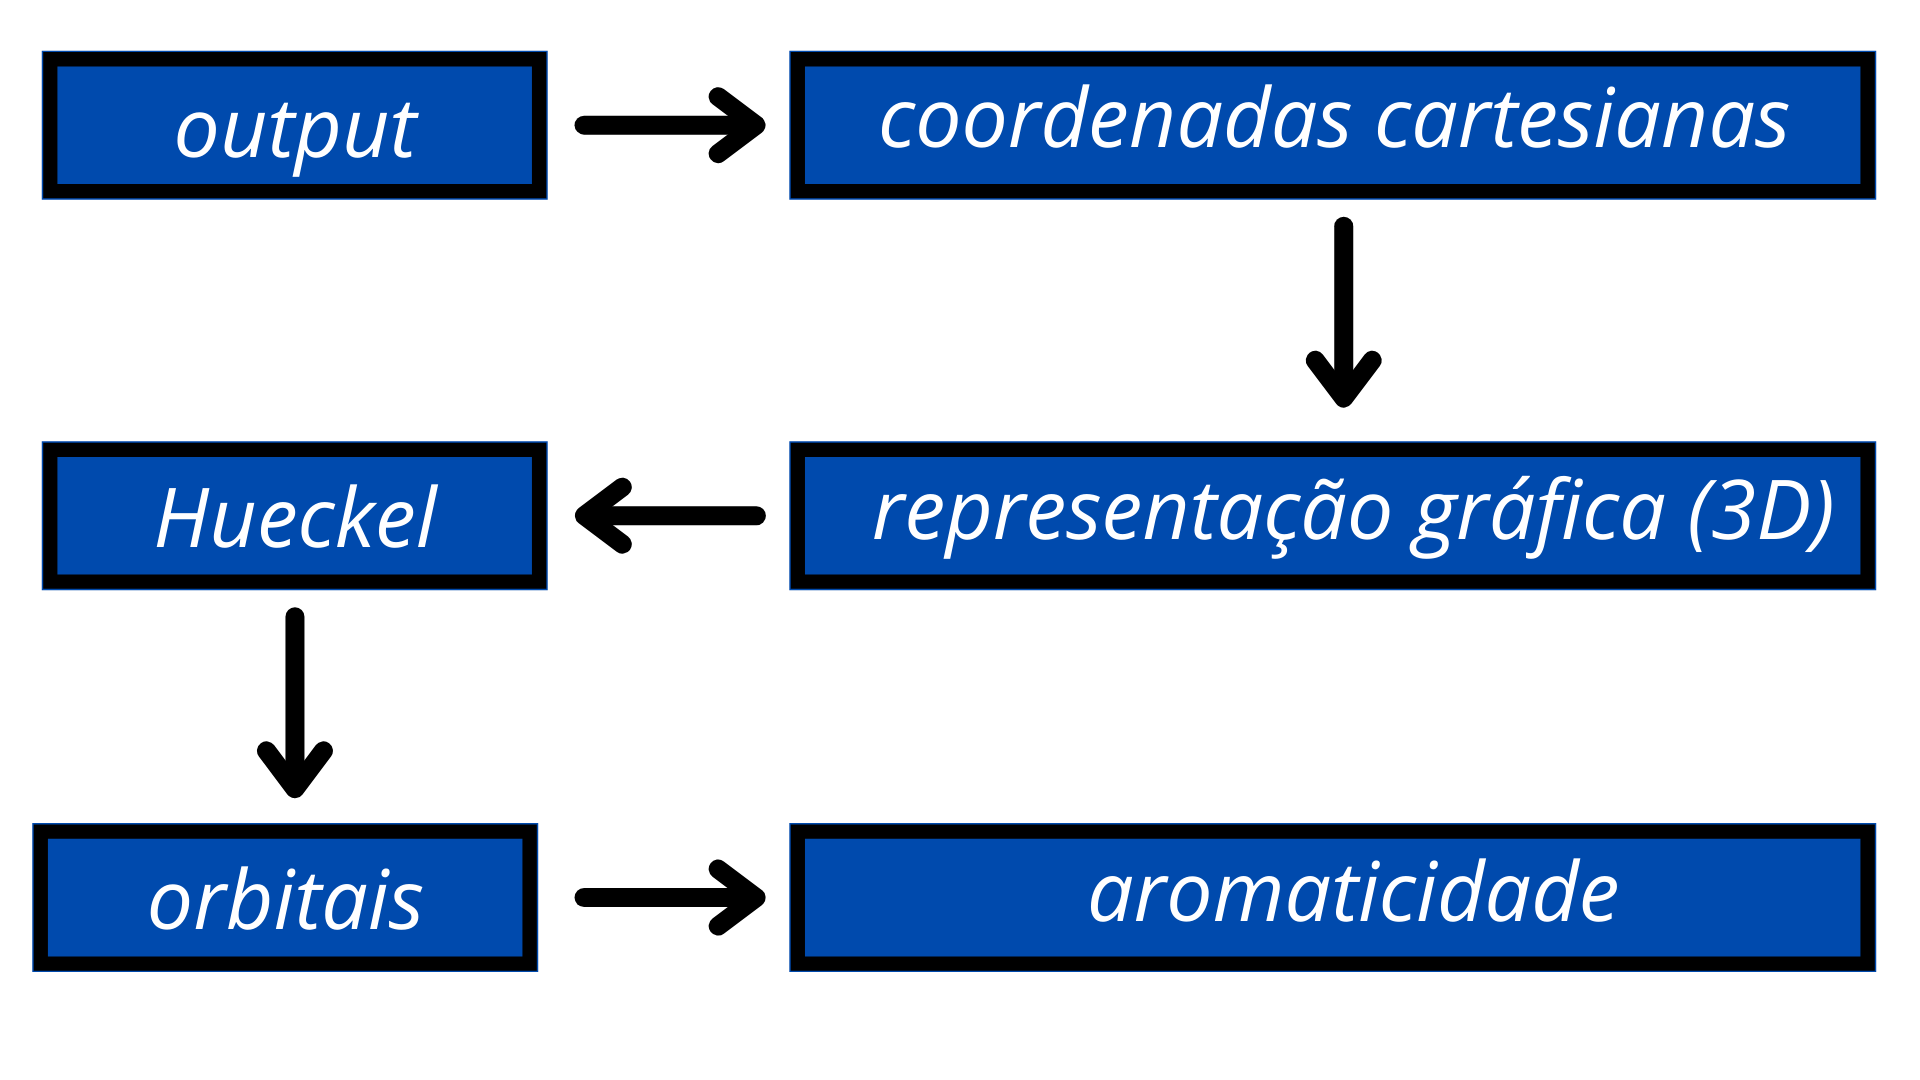
\includegraphics[width=0.6\textwidth]{images/workflow.png}
	\end{center}
	\fonte{Autor(a)}
\end{figure}

\begin{figure}[htb]
	\caption{\label{gui-pronta} Aqui é mostrada a interface gráfica produzida. Os círculos sinalizam as funções associadas às áreas da \gls{GUI}.}
	\begin{center}
		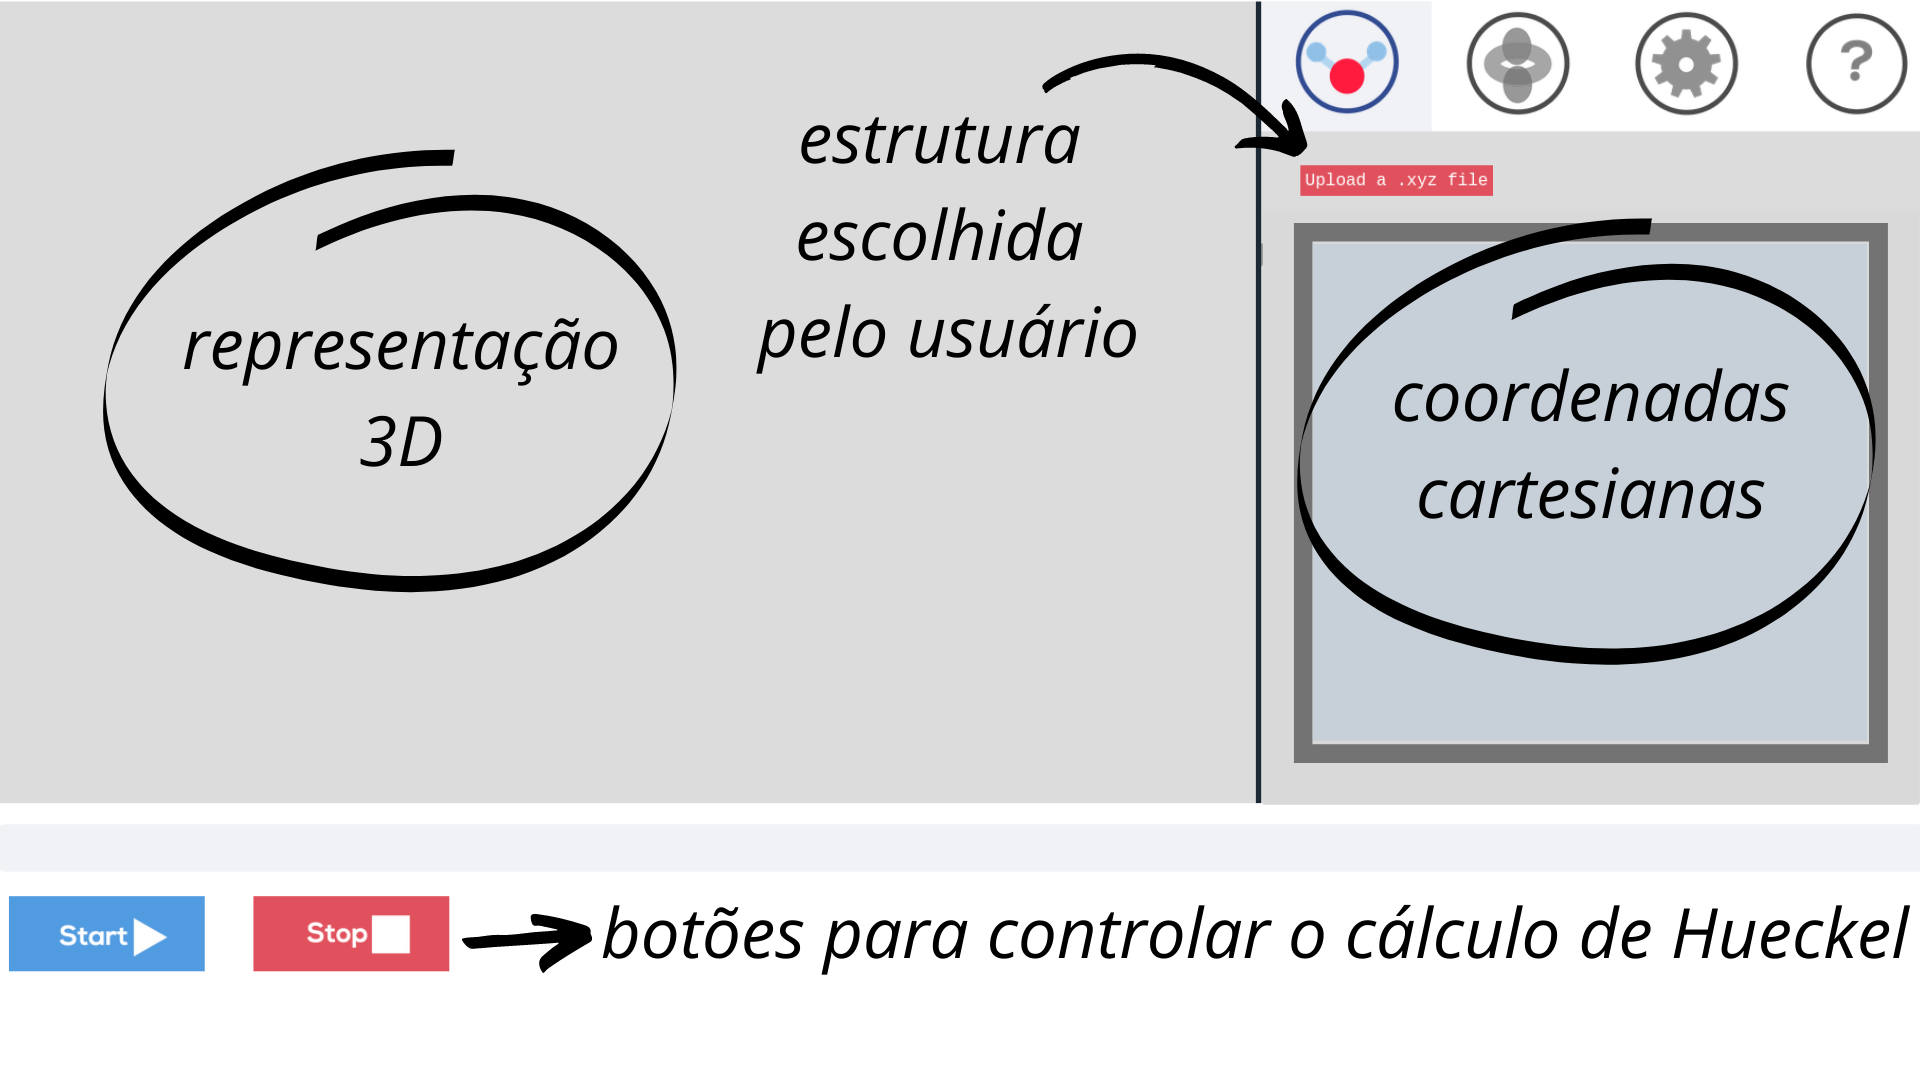
\includegraphics[width=0.8\textwidth]{images/GUI-EXAMPLE.png}
	\end{center}
	\fonte{Autor(a)}
\end{figure}

O fluxo de trabalho básico de funcionamento do \textit{Balmy.jl} também é ilustrado pelo esquema da \autoref{workflow}, onde é possível notar que o usuário insere, como entrada, o arquivo contendo as coordenadas cartesianas do sistema químico que deseja estudar. A \autoref{fig:input} mostra um exemplo de \textit{input} do \textit{Balmy.jl} para a molécula de benzeno. É um arquivo de extensão \textit{.xyz} que contém as coordenadas cartesianas da molécula de interesse. Na primeira linha, temos o nome da estrutura, em seguida, um comentário, e a partir da terceira linha são mostradas as informações da geometria em quatro colunas. A primeira delas contém os símbolos dos átomos contidos na molécula. Da segunda à quarta coluna, são indicadas as coordenadas cartesianas do eixo $x$, $y$ e $z$, respectivamente. Esses dados aparecem na caixa de texto no lado direito da tela (espaço indicado na \autoref{gui-pronta}).

\begin{figure}[htb]
	\caption{\label{fig:input} Exemplo de um arquivo de \textit{input} (\textit{.xyz}) para o \textit{Balmy.jl}.}
	\begin{center}
		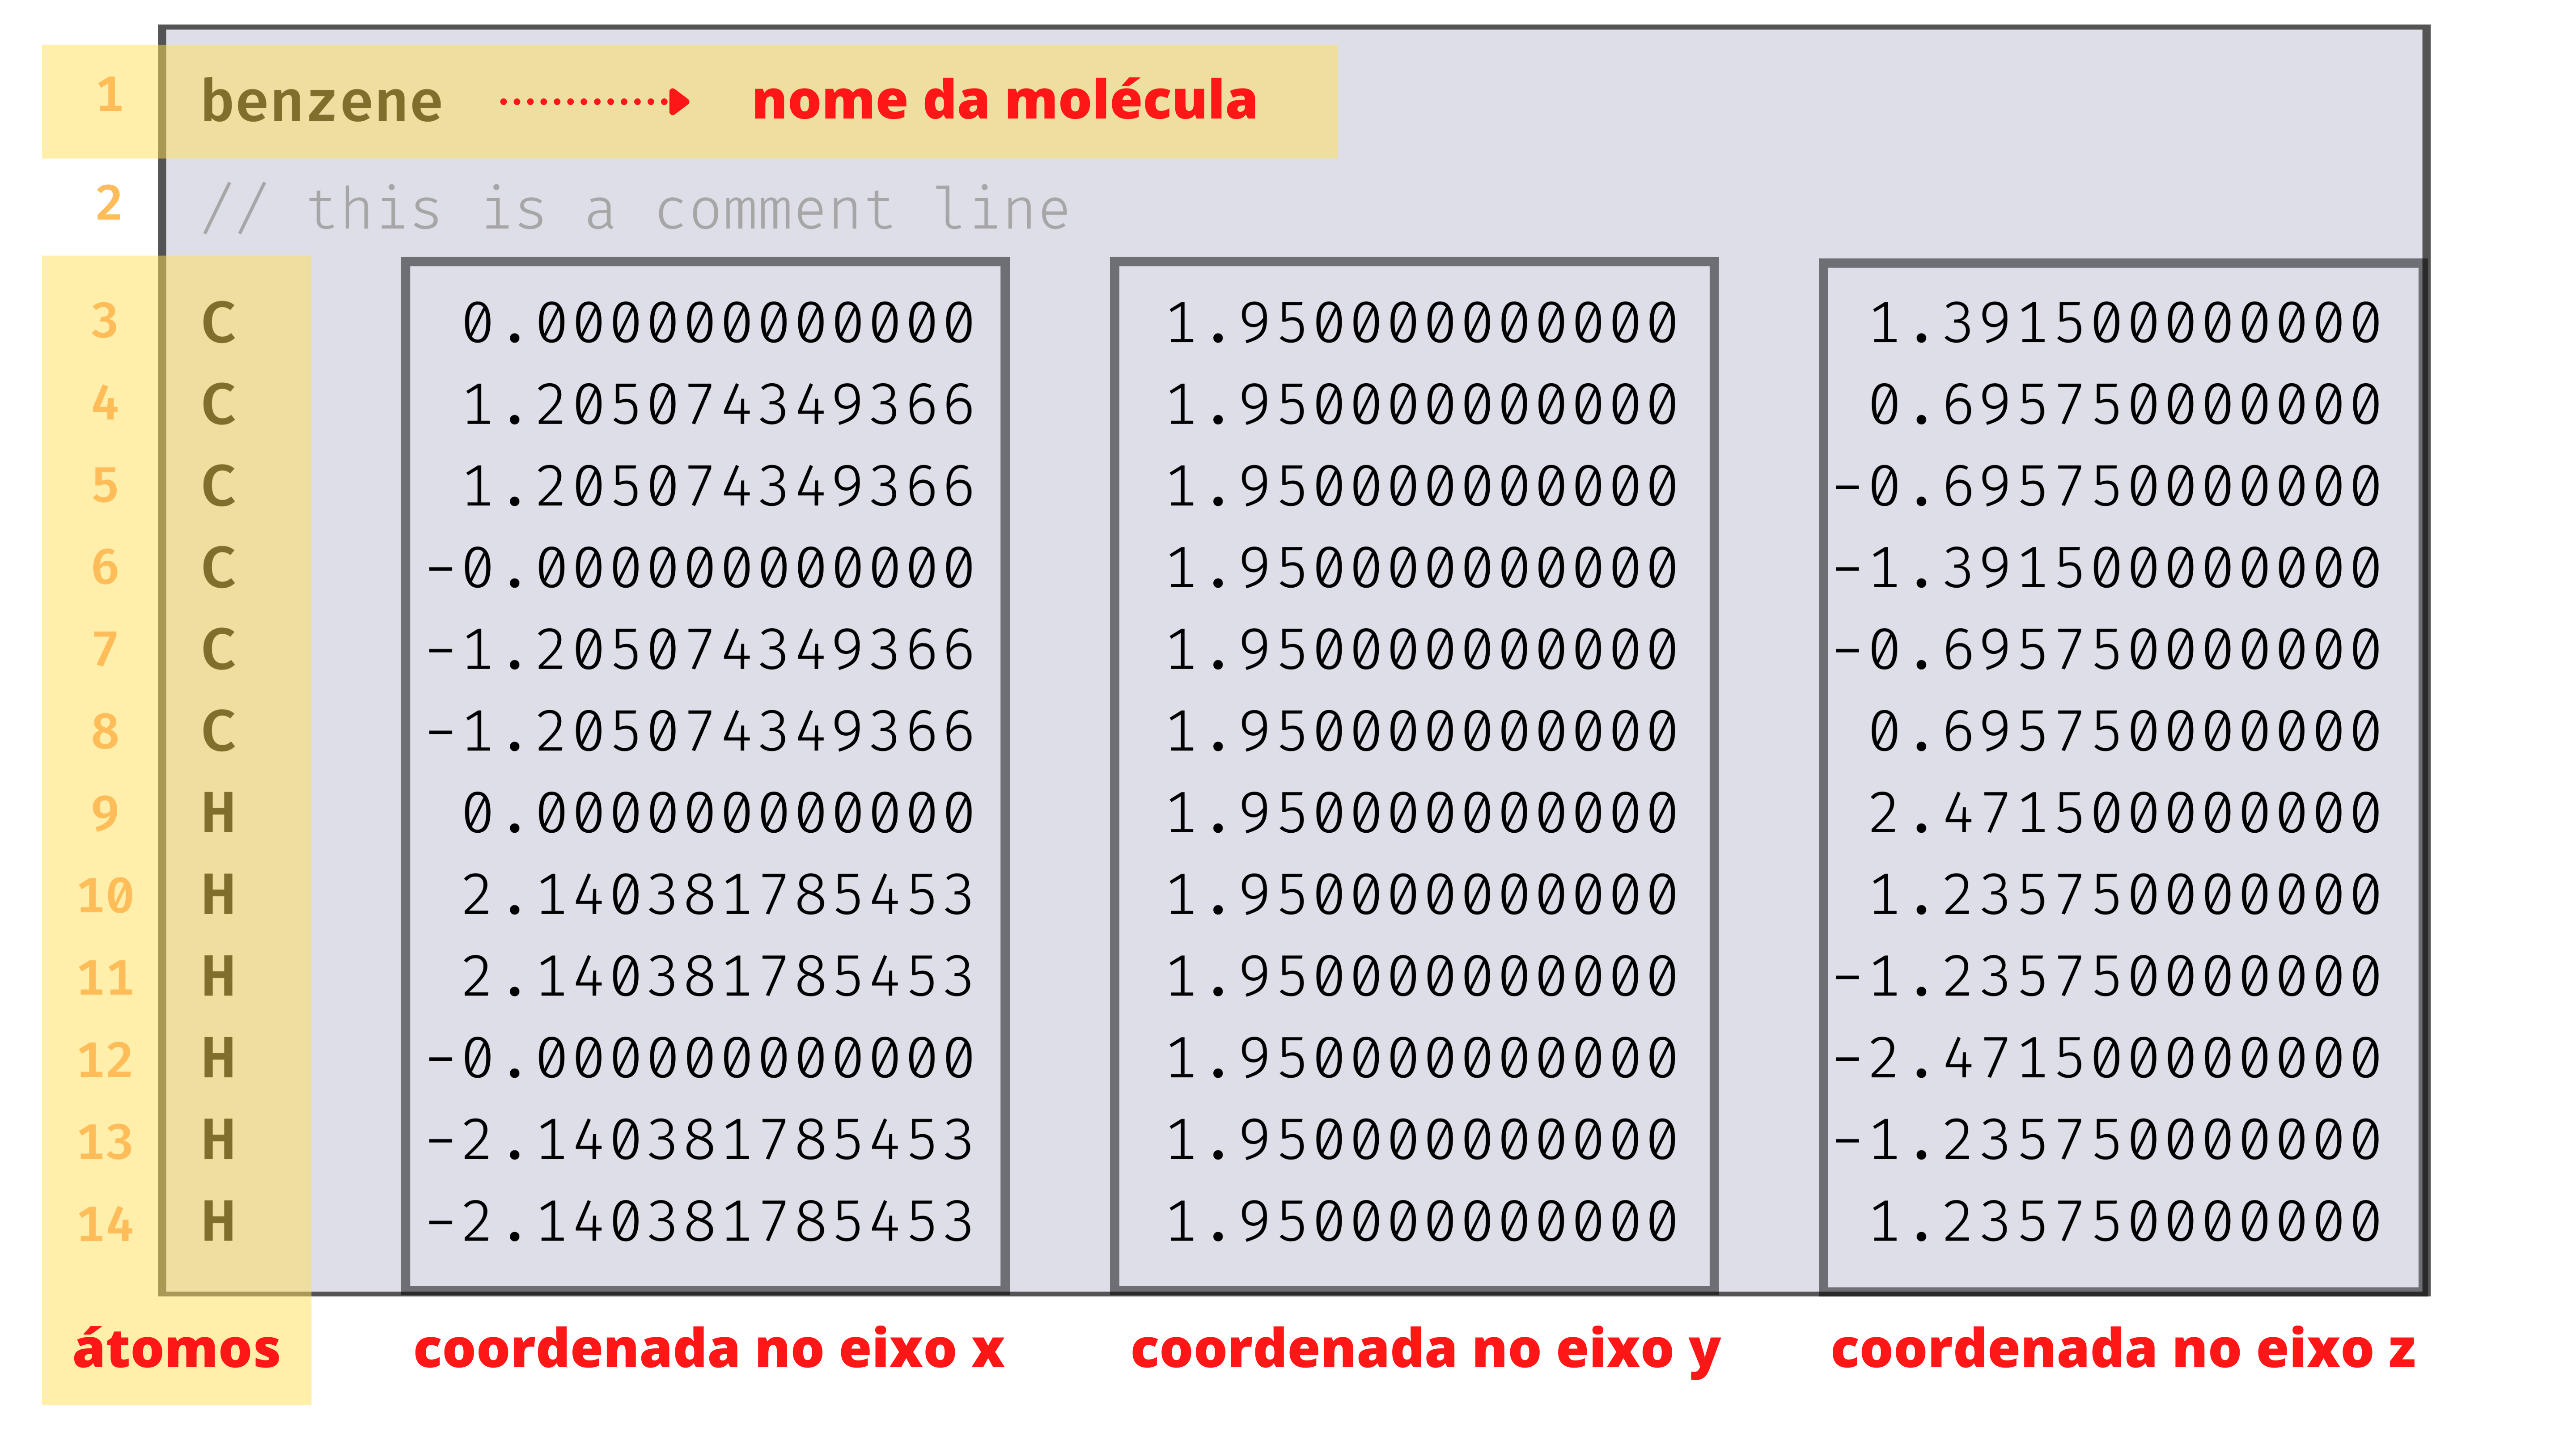
\includegraphics[width=0.8\textwidth]{images/fig2(4).png}
	\end{center}
	\fonte{Autor(a)}
\end{figure}

A partir das informações geométricas fornecidas pelo usuário, a estrutura é renderizada e representada tridimensionalmente pelo modelo das superfícies de Blinn-Phong (veja a \autoref{desenhoestrutural} para uma melhor descrição desse método). Nesse sentido, o \textit{Balmy.jl} é bastante versátil, pois é possível customizar o modelo através dos efeitos de iluminação empregados nas estruturas. Por exemplo, variando o valor de $\alpha'$ (coeficiente de brilho), é possível notar que, na \autoref{fig:representations}, quanto maior for o valor, menor será o holofote especular, representado pelos pontos luminosos nas estruturas moleculares.

%%% discutir equação do alpha

\begin{figure}[htb]
\caption{\label{fig:representations} Exemplo da aplicação do modelo de Blinn-Phong na molécula de benzenos a partir da alteração dos coeficientes $\alpha'$ para os átomos (representados por esferas). Da direita para a esquerda, os valores atribuídos foram: 0, 10, 50, 100, 1000; respectivamente.}
	\begin{center}
		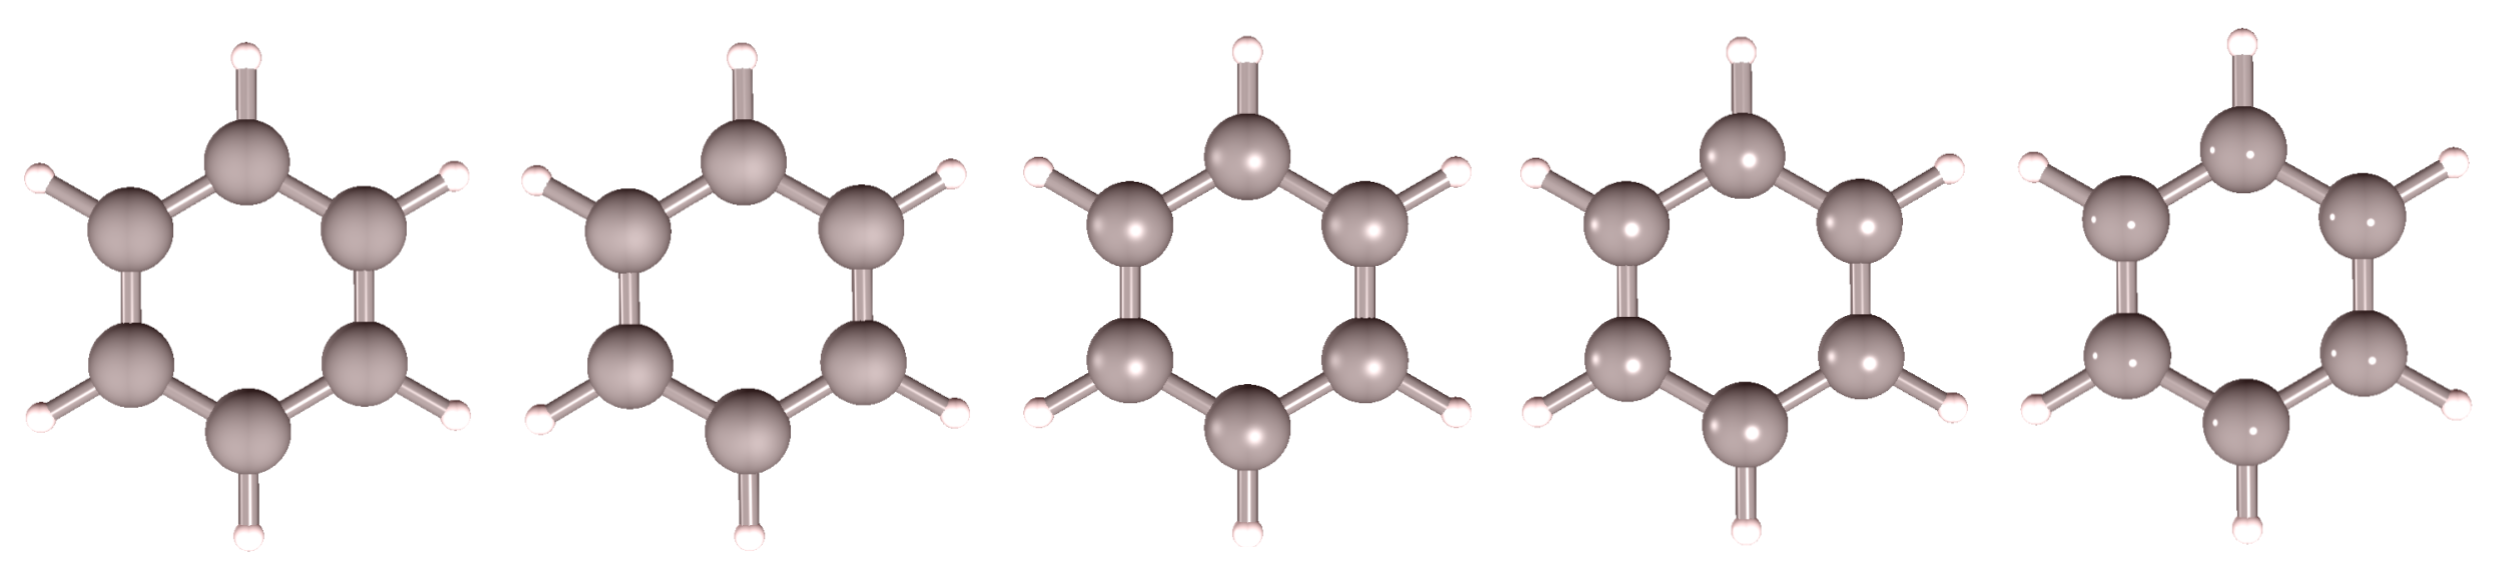
\includegraphics[width=1.0\textwidth]{images/shininess(1).png}
	\end{center}
	\fonte{Autor(a)}
\end{figure}

Antes da realização dos cálculos, é possível ainda acessar a terceira aba do \textit{Balmy.jl} para modificar o padrão das configurações (\autoref{fig:conf}). Por exemplo, é possível alterar a carga do composto (embora, por definição, o \textit{Balmy.jl} considere a moléula neutra) e o parâmetro de Wolfsberg-Helmholtz ($K$) (o padrão adotado é 1.75, parametrizado para hidrocarbonetos \autocite{Hoffmann1963}), que será discutido mais profundamente na \autoref{wolfsberg}.

\begin{figure}[htb]
	\caption{\label{fig:conf} Aqui, é mostrada a aba de configurações do cálculo realizado no \textit{Balmy.jl}}
	\begin{center}
		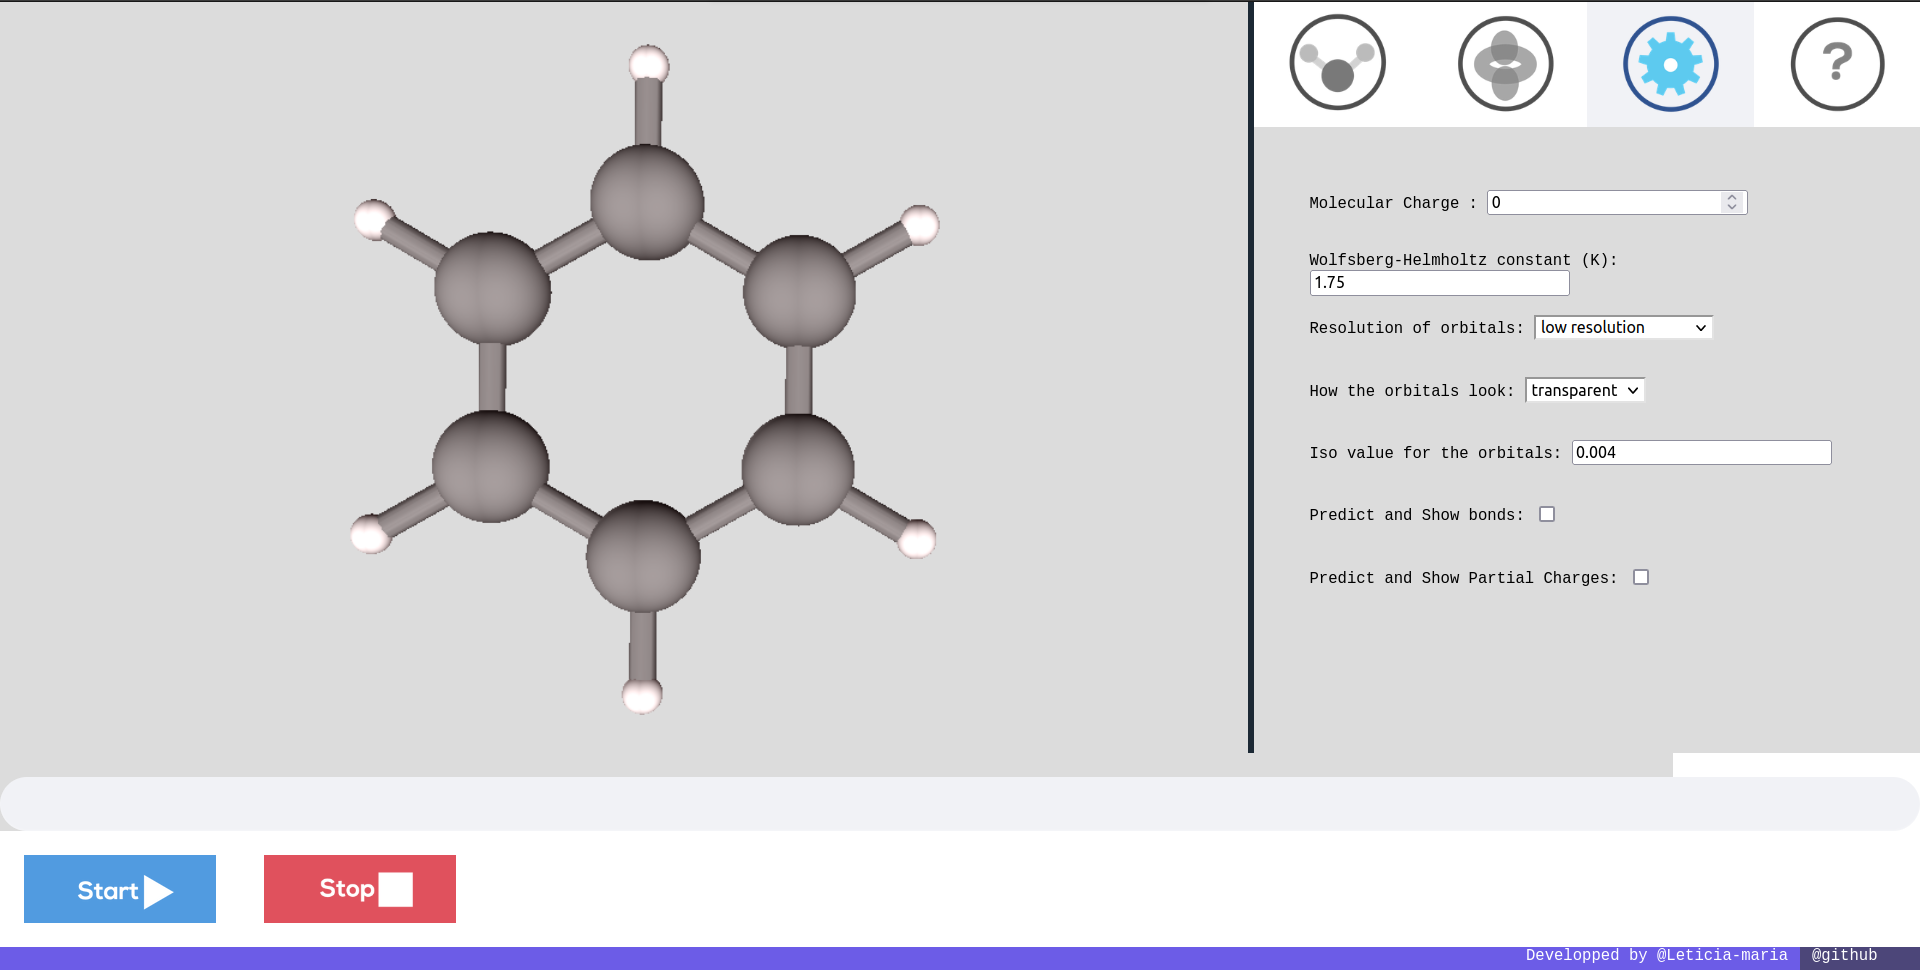
\includegraphics[width=0.8\textwidth]{images/conf.png}
	\end{center}
	\fonte{Autor(a)}
\end{figure}


Ao clicar no botão \textit{Start}, o usuário emite a requisição ao servidor para que o cálculo de \gls{EHMO} seja iniciado. Em questão de segundos, será possível acessar os resultados relativos ãs funções de onda e aos \gls{MOs} na segunda aba (\autoref{fig:results}). Para o caso do benzeno, os resultados serão discutidos na \autoref{sec:benzene}.

\begin{figure}[htb]
	\caption{\label{fig:results} Aqui, é mostrada a aba de resultados do cálculo realizado no \textit{Balmy.jl}}
	\begin{center}
		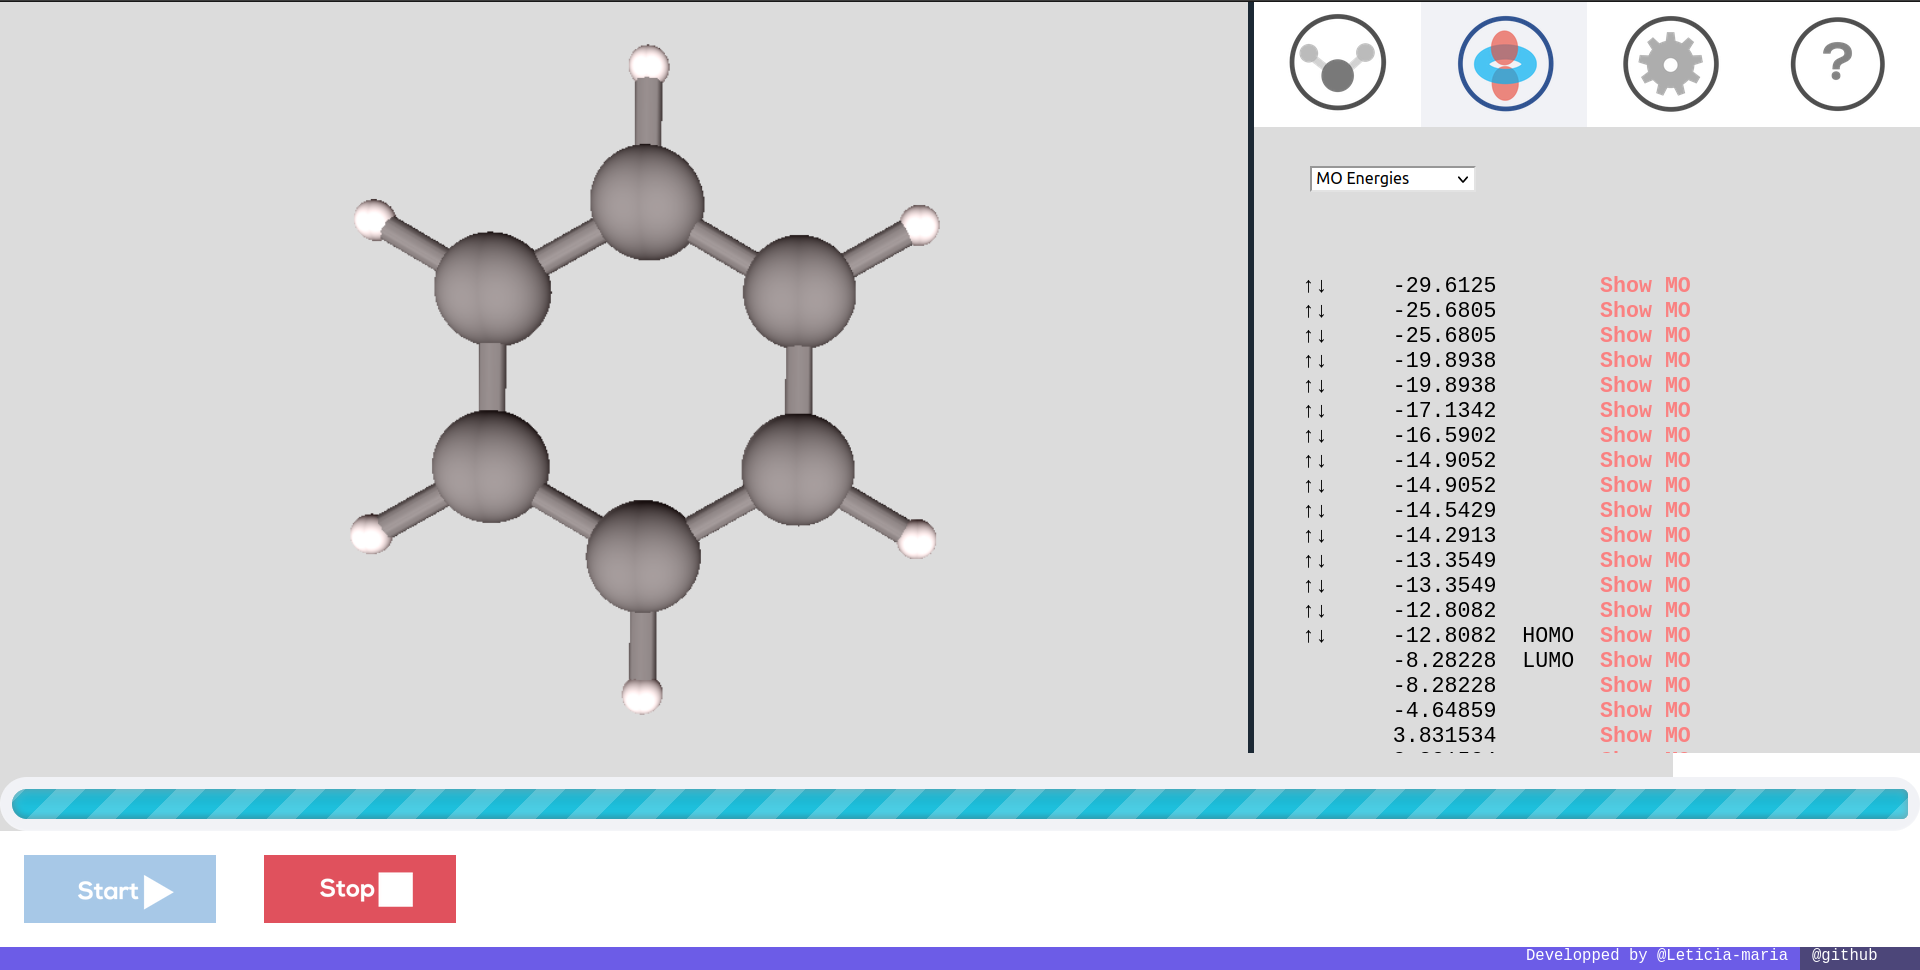
\includegraphics[width=0.8\textwidth]{images/results.png}
	\end{center}
	\fonte{Autor(a)}
\end{figure}

\section{Diagramas de orbitais moleculares}\label{sec:benzene}

Como o enfoque desse trabalho é a análise de compostos aromáticos, analisaremos de maneira mais aprofundada o exemplo do benzeno, cujas coordenadas estão mostradas na \autoref{tab:coords}. Os comprimentos de ligação obtidos para \ce{C-C} são $1.40$ \AA, e para \ce{C-H} são $1.10$ \AA.

\begin{table}[htb]
	\centering
	\caption{\label{tab:coords} Coordenadas atômicas do benzeno.}	
	\begin{tabular}{crrr}
		\toprule
		\textbf{Átomo (posição)} & coordenada $x$ & coordenada $y$ & coordenada $z$
		\\ 
		\midrule
C(1)  &    0.000000000000  &   1.950000000000  &   1.391500000000  \\
C(2)  &    1.205074349366  &   1.950000000000  &   0.695750000000  \\
C(3)  &    1.205074349366  &   1.950000000000  &  -0.695750000000  \\
C(4)  &   -0.000000000000  &   1.950000000000  &  -1.391500000000  \\
C(5)  &   -1.205074349366  &   1.950000000000  &  -0.695750000000  \\
C(6)  &   -1.205074349366  &   1.950000000000  &   0.695750000000  \\
H(1)  &    0.000000000000  &   1.950000000000  &   2.471500000000  \\
H(2)  &    2.140381785453  &   1.950000000000  &   1.235750000000  \\
H(3)  &    2.140381785453  &   1.950000000000  &  -1.235750000000  \\
H(4)  &   -0.000000000000  &   1.950000000000  &  -2.471500000000  \\
H(5)  &   -2.140381785453  &   1.950000000000  &  -1.235750000000  \\
H(6)  &   -2.140381785453  &   1.950000000000  &   1.235750000000  \\
    \bottomrule
	\end{tabular}
	\fonte{Autor(a).}
\end{table}

Seguindo o grafo mostrado na \autoref{fig:M2} e enumerado na \autoref{fig:graphEnumerated}, é possível construir uma matriz de adjacência de dimensão $n \times n$, onde $n$ é o número de átomos, excluindo-se os hidrogênios. No caso do benzeno, a ordem da matriz em questão é 6.

\begin{figure}[htb]
\vspace{0.8\baselineskip}
\begin{equation}
\label{eq:adjmatrix}
\begin{bmatrix}
    0 & 1 & 0 & 0 & 0 & 1 \\
    1 & 0 & 1 & 0 & 0 & 0 \\
    0 & 1 & 0 & 1 & 0 & 0 \\
    0 & 0 & 1 & 0 & 1 & 0 \\
    0 & 0 & 0 & 1 & 0 & 1 \\
    1 & 0 & 0 & 0 & 1 & 0
\end{bmatrix}
\end{equation}
\end{figure}

\noindent Consideremos $a_{ij}$ o elemento geral associado à matriz da \autoref{eq:5}, sendo igual a uma unidade quando os carbonos $i$ e $j$ estão ligados. Analogamente, na teoria de Hueckel e de Hueckel estendido, a matriz do determinante secular (\autoref{eq:secularmatrix}) é aquela cujos autovalores determinam as energias dos orbitais moleculares.

\begin{figure}[htb]
\vspace{0.8\baselineskip}
\begin{equation}
\label{eq:secularmatrix}
\begin{bmatrix}
    \alpha - E & \beta & 0 & 0 & 0 & \beta \\
    \beta & \alpha - E & \beta & 0 & 0 & 0 \\
    0 & \beta & \alpha - E & \beta & 0 & 0 \\
    0 & 0 & \beta & \alpha - E & \beta & 0 \\
    0 & 0 & 0 & \beta & \alpha - E & \beta \\
    \beta & 0 & 0 & 0 & \beta & \alpha - E \\
\end{bmatrix}
\end{equation}
\end{figure}

No caso do benzeno, ao resolver o determinante secular da matriz anterior (através do procedimento mostrado no \autoref{ap:HMO} e no \autoref{ap:EHMO}), obtemos a equação

\begin{figure}[htb]
\begin{equation}
    \label{eq:R3}
    \tikzmarknode{variable}{\highlight{blue}{$x$}}^6 - 6\highlight{blue}{$x$}^4 + 9\highlight{blue}{$x$}^2 = 0
\end{equation}
\begin{tikzpicture}[overlay,remember picture,>=stealth,nodes={align=left,inner ysep=1pt},<-]
    \path (variable.south) ++ (1,-1.5em) node[anchor=north west,color=blue!67] (scalep){\textit{$x = \displaystyle \frac{\alpha - E}{\beta}$}};
    \draw [color=blue!87](variable.south) |- ([xshift=1.65em,color=blue]scalep.north east);
\end{tikzpicture}
\vspace{2\baselineskip}
\end{figure}

\begin{figure}[htb]
\vspace{2\baselineskip}
\begin{equation}
    \label{eq:orb_mols}
\begin{split}
    \tikzmarknode{e1}{\highlight{blue}{$E_1$}} = \alpha +  2 \beta \\[0.3cm]
    \tikzmarknode{e2}{\highlight{red}{$E_2 = E_3$}} = \alpha + \beta \\
    \tikzmarknode{e3}{\highlight{red}{$E_4 = E_5$}} = \alpha - \beta \\[0.3cm]
    \tikzmarknode{e6}{\highlight{blue}{$E_6$}} = \alpha - 2\beta
\end{split}
\end{equation}
\begin{tikzpicture}[overlay,remember picture,>=stealth,nodes={align=left,inner ysep=1pt},<-]
    \path (e1.north) ++ (1,1.5em) node[anchor=south west,color=blue!67] (scalep){\textit{HOMO-1}};
    \draw [color=blue!87](e1.north) |- ([xshift=1.65em,color=blue]scalep.south east);

    \path (e2.north) ++ (-0.60,0.6em) node[anchor=south east,color=red!67] (scalep){\textit{HOMO (orbitais degenerados)}};
    \draw [color=red!87](e2.north) |- ([xshift=-1.65em,color=red]scalep.south west);
    
    \path (e3.south) ++ (-0.60,-0.6em) node[anchor=north east,color=red!67] (scalep){\textit{LUMO (orbitais degenerados)}};
    \draw [color=red!87](e3.south) |- ([xshift=-1.65em,color=red]scalep.north west);
    
    \path (e6.south) ++ (1,-1.5em) node[anchor=north west,color=blue!67] (scalep){\textit{LUMO+1}};
    \draw [color=blue!87](e6.south) |- ([xshift=1.65em,color=blue]scalep.north east);
\end{tikzpicture}
\end{figure}

Resolvendo o polinômio da \autoref{eq:R3}, conseguimos suas raízes ($x = \pm 1, \pm 1, \pm 2$) e, portanto, as energias para seis orbitais moleculares do benzeno (HOMO-1, HOMO, LUMO, LUMO+1). Combinando as raízes com os parâmetros $\alpha$ e $\beta$, nós temos a \autoref{eq:orb_mols} (\autoref{fig:MOs}).

\begin{figure}[htb]
\caption{\label{fig:MOs} Diagrama de energia dos orbitais moleculares do benzeno.}
	\begin{center}
		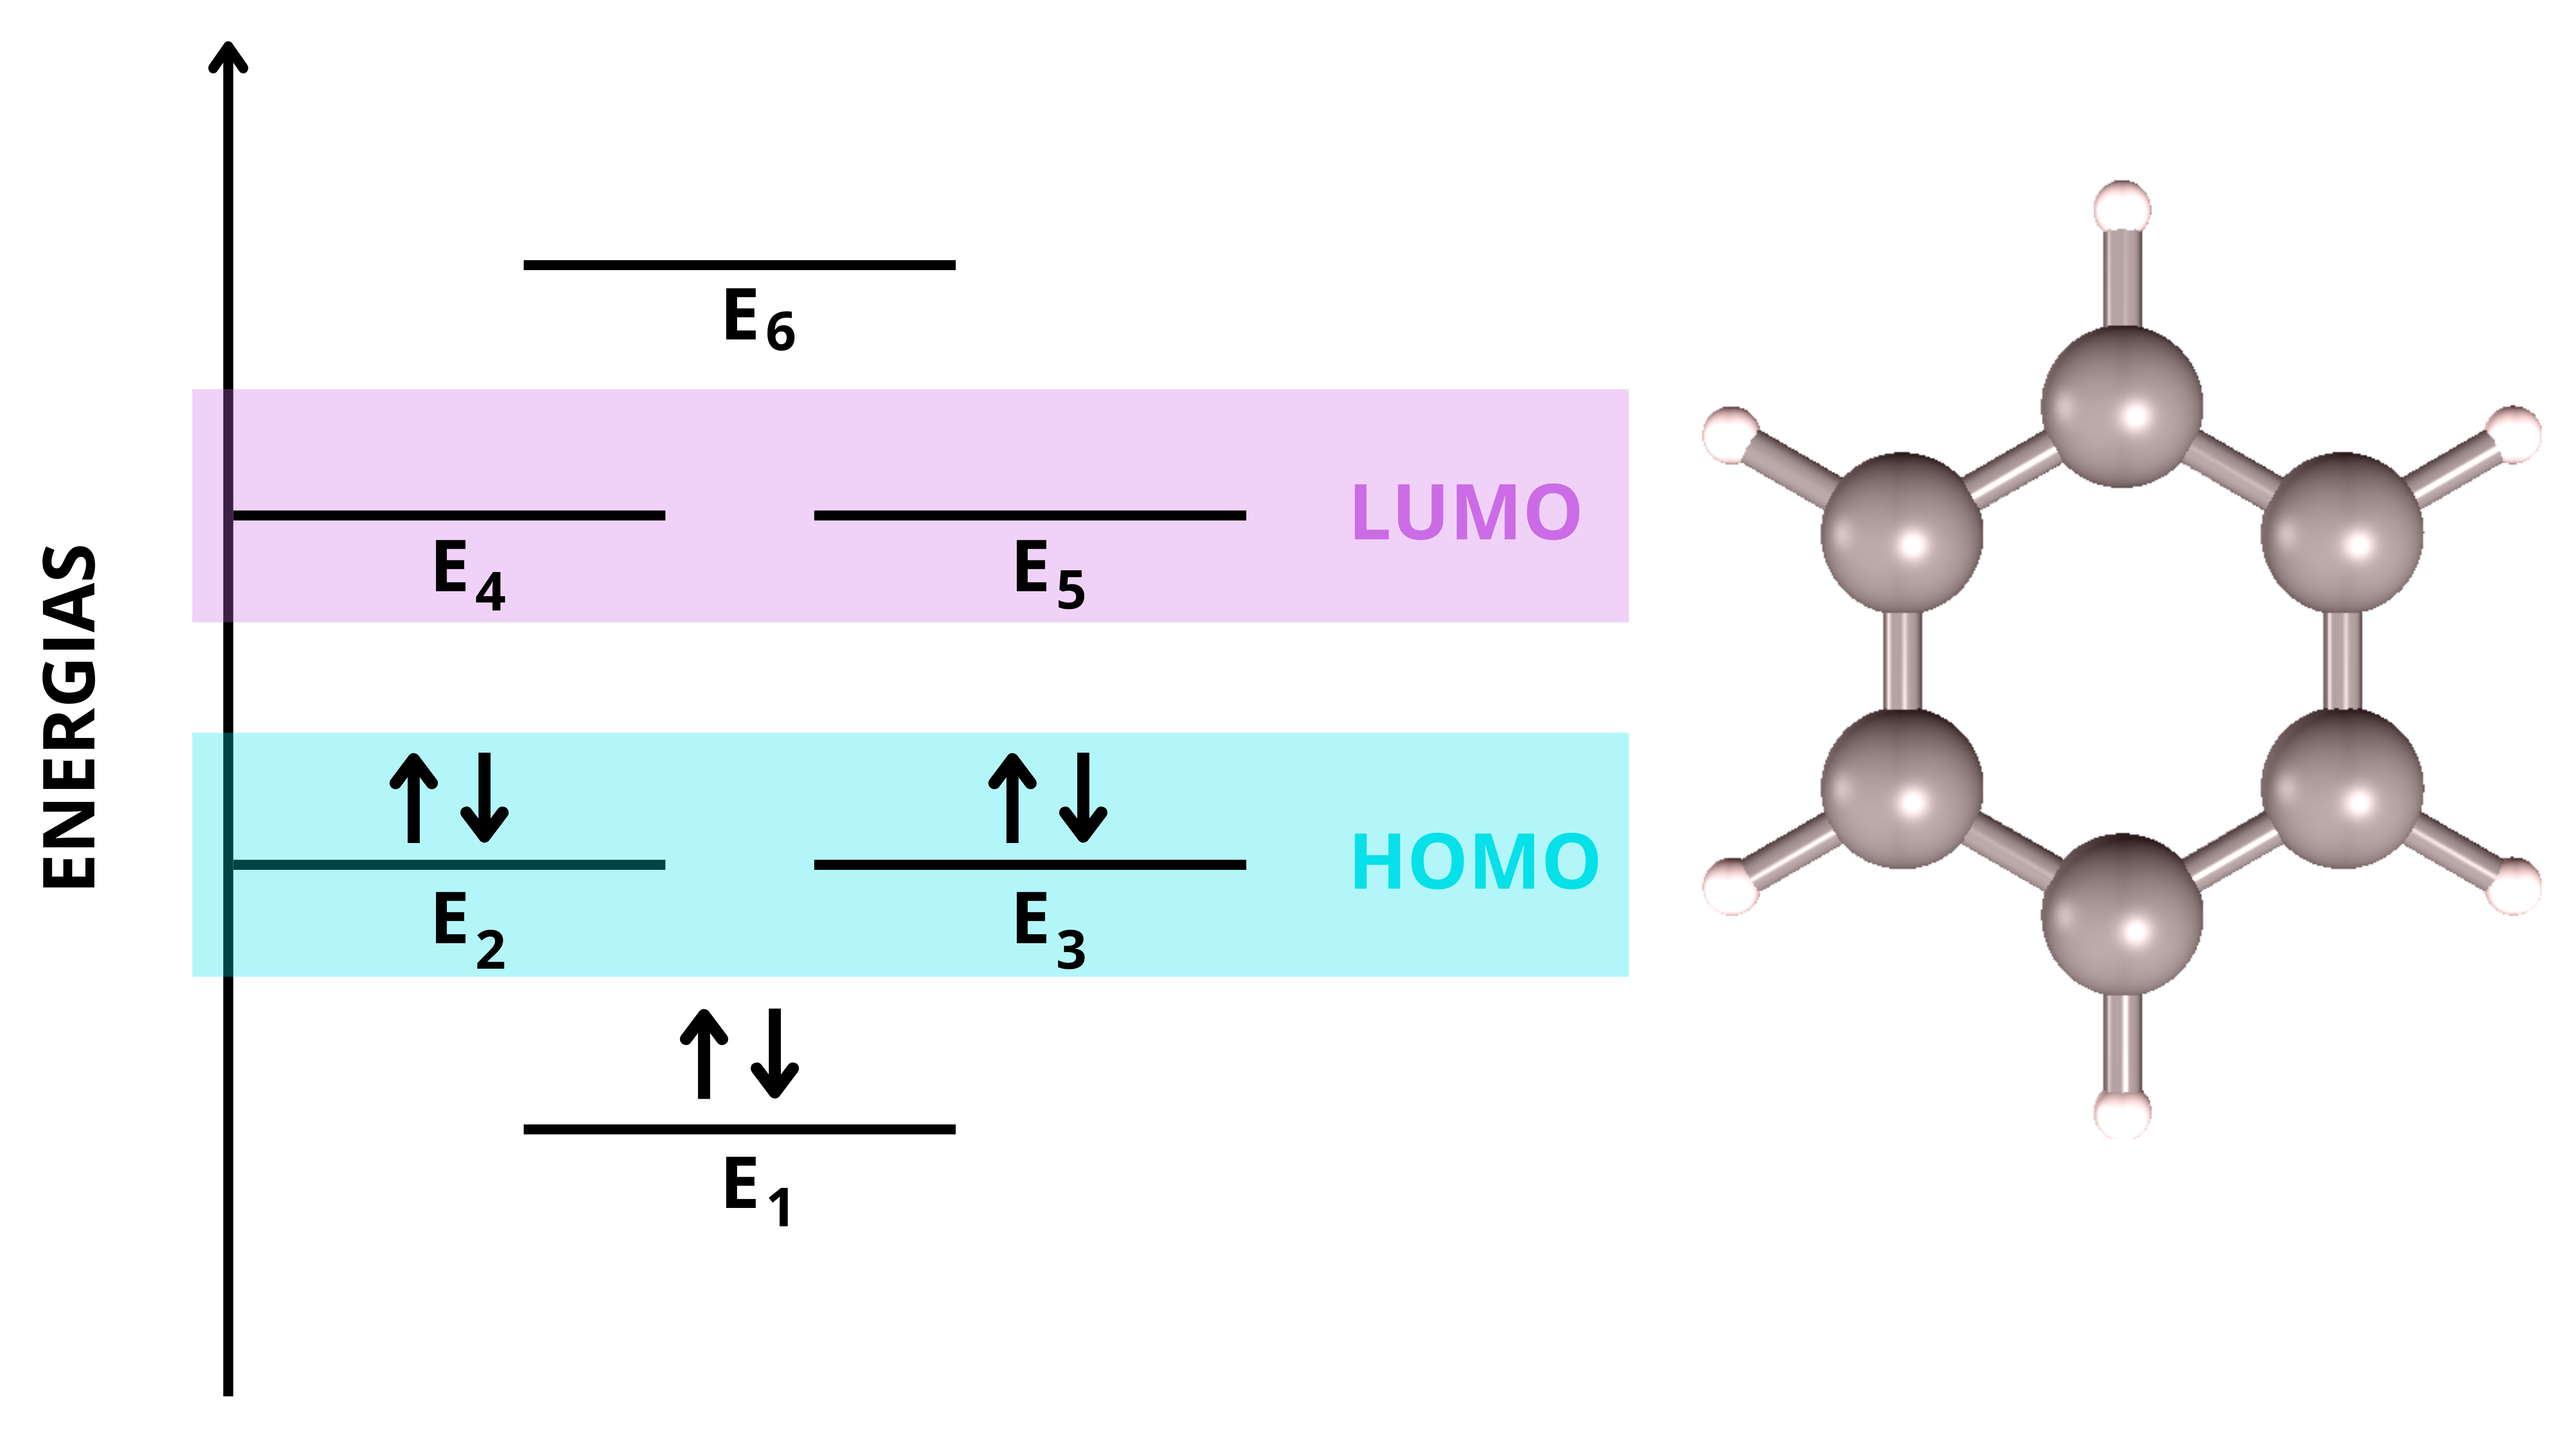
\includegraphics[width=0.75\textwidth]{images/MOs.png}
	\end{center}
	\fonte{Autor(a).}
\end{figure}

Os autovalores repetidos vão gerar orbitais degenerados, isto é, aqueles que estão no mesmo nível energético, como é possível notar no diagrama e nos valores de energia obtidos. Esses mesmos valores podem ser obtidos se calcularmos os autovalores da matriz de adjacência. Desse modo, comprovamos que, ao solucionar o determinante e os autovalores da matriz secular, é possível obter os valores de energia e as populações associadas a cada orbital molecular da molécula de interesse.

O diagrama de níveis de energia para o benzeno é dado na \autoref{fig:MOs}. Os seis elétrons $\pi$ são colocados nos três níveis de energia mais baixos. Desse modo, a energia eletrônica em benzeno é definida pela \autoref{epi}.

\begin{equation}
\label{epi}
    E_\pi = 2(\alpha + 2\beta) + 4(\alpha + \beta) = 6\alpha + 8\beta
\end{equation}

As funções de onda resultantes para os seis orbitais moleculares $\pi$ do benzeno são dados pela \autoref{wavefunctions}.

\begin{equation}
\label{wavefunctions}
\begin{split}
    \psi_1 = \frac{1}{\sqrt{6}}(2p_{z1} + 2p_{z2} + 2p_{z3} + 2p_{z4} + 2p_{z5} + 2p_{z6}) \Longrightarrow E_1 = \alpha + 2\beta \\
    \psi_2 = \frac{1}{\sqrt{4}}(2p_{z2} + 2p_{z3} - 2p_{z5} - 2p_{z6}) \Longrightarrow E_2 = \alpha + \beta \\
   \psi_3 = \frac{1}{\sqrt{3}}(2p_{z1} + \frac{1}{2} 2p_{z2} - \frac{1}{2} 2p_{z3} - 2p_{z4} - \frac{1}{2} 2p_{z5} + \frac{1}{2} 2p_{z6}) \Longrightarrow E_3 = \alpha + \beta \\
     \psi_4 = \frac{1}{\sqrt{4}}(2p_{z2} - 2p_{z3} + 2p_{z5} - 2p_{z6}) \Longrightarrow E_4 = \alpha - \beta \\
      \psi_5 = \frac{1}{\sqrt{3}}(2p_{z1} - \frac{1}{2} 2p_{z2} - \frac{1}{2} 2p_{z3} + 2p_{z4} - \frac{1}{2} 2p_{z5} - \frac{1}{2} 2p_{z6}) \Longrightarrow E_5 = \alpha - \beta \\
      \psi_6 = \frac{1}{\sqrt{6}}(2p_{z1} - 2p_{z2} + 2p_{z3} - 2p_{z4} +  2p_{z5} -  2p_{z6}) \Longrightarrow E_6 = \alpha - 2\beta 
\end{split}
\end{equation}


\begin{table}[htb]
	\centering
	\caption{\label{qua:Quadro_1} Energias dos orbitais de fronteira de alguns hidrocarbonetos aromáticos.}	
	\begin{tabular}{lrrr}
		\toprule
		\textbf{Molécula} & \textbf{HOMO/(eV)} & \textbf{LUMO/(eV)} & \textbf{Gap/(eV)}
		\\ 
		\midrule
        benzeno & -12.808 & -8.282 & 4.452 \\
        naftaleno & -12.073 & -9.338 & 2.635 \\
        antraceno & -11.642 & -9.839 & 1.803 \\
        fenantreno & -12.023 & -9.310 & 2.713 \\
        azuleno & -11.730 & -9.872 & 1.858 \\
        pentaleno & -11.492 & -10.809 & 0.683 \\
        fulveno & -11.991 & -10.338 & 1.653 \\
        bifenileno & -11.555 & -9.553 & 2.002 \\
        tolueno & -12.502 & -8.348 & 4.154 \\
    \bottomrule
	\end{tabular}
	\fonte{Autor(a).}
\end{table}

\section{Hidrocarbonetos aromáticos}

Analisando os dados da \autoref{tab:energies}, concluímos que a ordem das estabilidades dos compostos está de acordo com aqueles apresentados por Hoffmann \autocite{Hoffmann1963}, e com os dados experimentais publicados por Heilbronner \autocite{ginsburg1959}. Por exemplo, o naftaleno mostra-se 32.3 kcal/mol mais estável do que o azuleno, o que é um ótimo resultado se comparado com o valor de referência (32.6 kcal/mol)\autocite{ginsburg1959}. O fulveno, por sua vez, é computado como sendo 25.6 kcal/mol menos estável do que o benzeno, em relação ao valor de 27 kcal/mol tomado como modelo\autocite{CHENG1956}. O antraceno, por sua vez, é 4.2 kcal/mol mais estável do que o fenantreno, enquanto o último isômero é, na verdade, 6.9 kcal/mol mais estável \autocite{Hoffmann1963}, o que provém do fato de que há repulsão estérica entre os hidrogênios do fenantreno.

\begin{table}[htb]
	\centering
	\caption{\label{tab:energies} Energias dos elétrons $\pi$ nos compostos aromáticos.}	
	\begin{tabular}{lrr}
		\toprule
		\textbf{Molécula} & $E_\pi / (eV)$ & $E_\pi / (kcal/mol)$
		\\ 
		\midrule
        Etileno & -26.336 & -609.628 \\
        Butadieno & -52.964 & -1221.38 \\
        Benzeno & -80.208 & -1849.64 \\
        Fulveno & -78.928 & -1820.12 \\
        Naftaleno & -133.676 & -3082.64 \\
        Azuleno & -132.934 & -3065.53 \\
        Fenantreno & -187.286 & -4318.92 \\
        Antraceno & -187.020 & -4312.78 \\
    \bottomrule
	\end{tabular}
	\fonte{Autor(a).}
\end{table}

\section{Influência de K}\label{wolfsberg}


\section{Performance}

Para testar a performance da implementação do cálculo de \gls{EHMO} no \textit{Balmy.jl}, foi feita a comparação dos tempos de execução para os cálculos das energias eletrônicas. O tamanho do sistema químico avaliado foi variado com base na estrutura do polietileno. Partiu-se do monômero (que contém 4 orbitais atômicos em seu conjunto de bases) até uma estrutura com grau de polimerização igual a 1250 (que contém 10000 orbitais atômicos em seu conjunto de bases). O resultado está mostrado na \autoref{fig:times}.

\begin{figure}[htb]
\caption{\label{fig:times} Gráfico da relação entre o número de bases da estrutura e o tempo de execução, em milisegundos (ms).}
	\begin{center}
		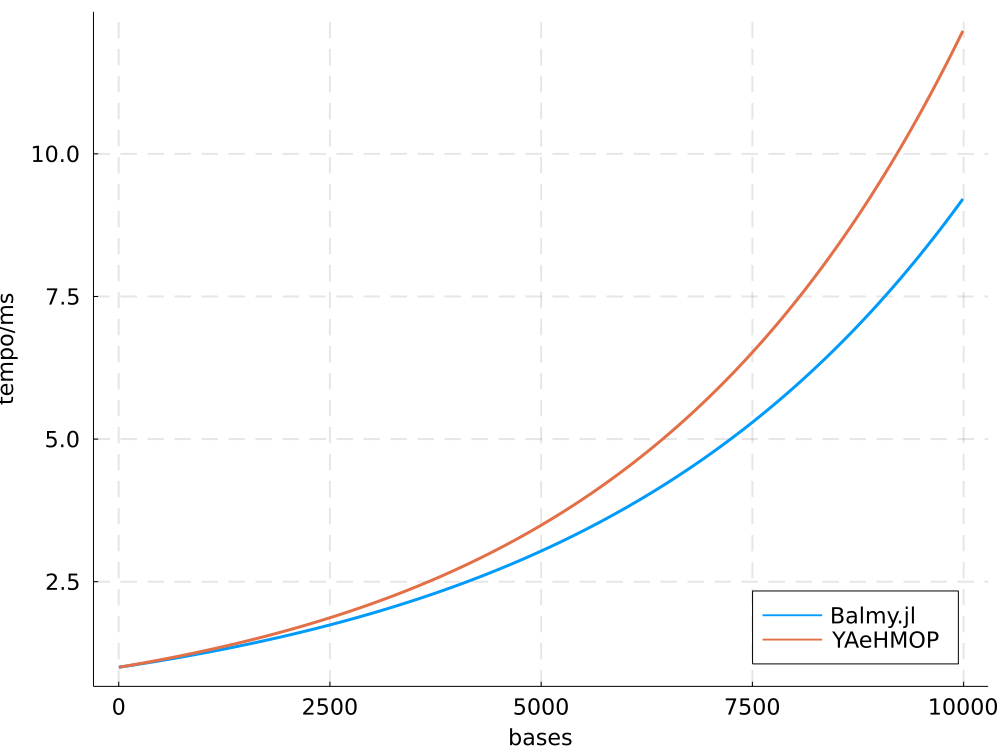
\includegraphics[width=0.75\textwidth]{images/tttt.png}
	\end{center}
	\fonte{Autor(a).}
\end{figure}

O perfil do gráfico mostra que o custo computacional para o cálculo da energia de uma molécula pode crescer exponencialmente. Comparando as duas curvas, ajustadas de acordo com a função exponencial, nota-se que há um ganho de tempo no uso do \textit{Balmy.jl} em relação ao \gls{YAeHMOP} conforme as estruturas de entrada crescem, que é escrito em linguagem C, que também é compilada. Isso ocorre pois, no código do \textit{Balmy.jl}, são implementadas otimizações inerentes à linguagem de programação Julia, como o dispacho múltiplo, que torna mais rápida a execução de funções matemáticas, junto à associação com \textit{macros}, que torna mais eficientes as iterações ao computar integrais.

\section{Índices geométricos}

Além dos orbitais moleculares e das funções de onda, o \textit{Balmy.jl} também permite analisar o \gls{HOMA}. Esse índice geométrico de aromaticidade foi modelado de acordo com uma escala normalizada pelo fator $\alpha$ (\autoref{eq:3}), onde o benzeno seria a referência de \textit{aromaticidade perfeita}, tendo \gls{HOMA} $=1$, pois o desvio entre os comprimentos de ligação individuais ($R_i$) e o comprimento ótimo de ligação ($R_{opt}$) (\autoref{eq:2}) é nulo. Isso faz com que os termos $EN$ e $GEO$, que diminuem a aromaticidade, sejam iguais a $0$.

\begin{equation}
    HOMA = 1 - EN - GEO \Longrightarrow HOMA = 1 - 0 - 0 \Longrightarrow HOMA = 1
\end{equation}

\begin{table}[htb]
	\centering
	\caption{\label{tab:ccbc} Comprimentos de ligação entre átomos de carbono. Como notação, adotamos a simbologia \ce{C-C} para representar a ligação simples, \ce{C=C} para a ligação dupla, \ce{C\simeq C} para representar a ligação CC aromática na molécula do benzeno.}	
	\begin{tabular}{ccc}
		\toprule
		\textbf{Tipo de ligação} & \textbf{Energia de ligação} & \textbf{Comprimento de ligação} \\
		\midrule
         \ce{C-C}  & 345 kJ/mol & 1.53 \AA \\
         \ce{C=C} & 612 kJ/mol & 1.34 \AA \\
         \ce{C\simeq C} & 420 kJ/mol & 1.40 \AA \\
    \bottomrule
	\end{tabular}
	\fonte{Autor(a).}
\end{table}

Por outro lado, \gls{HOMA} $= 0$ para o cicloexatrieno hipotético (\autoref{fig:2}), composto por ligações simples e duplas, sem deslocalização. Pode-se facilmente deduzir isso através da substituição dos valores da \autoref{tab:ccbc} na \autoref{eq:4}.

\begin{equation}
    \begin{split}
        HOMA = 1 - \bigg\{ \frac{98.89}{6} \{ 3[(1.40 - R_{\ce{C-C}})^2] + 3[(1.40 - R_{\ce{C=C}})^2] \} \bigg\} \\
        HOMA = 1 - \bigg\{ \frac{98.89}{6} \{ 3[(1.40 - 1.53)^2] + 3[(1.40 - 1.34)^2] \} \bigg\} \\
        HOMA = 1 - \bigg[ \frac{98.89}{6} (0.0615) \bigg] \\
        HOMA = 1 - 1 = 0
    \end{split}
\end{equation}

%Ou seja, a ideia original e fundamental é que cada par de átomos pode ser envolvido em ambas as ligações $\sigma$ e $\pi$, com $R_\sigma > R_\pi$. A distância de ligação $R_i$ representa uma compressão de $R_\sigma$ e uma extensão de $R_\pi$.

\subsection{Hidrocarbonetos policíclicos aromáticos}

O arquivo de saída gerado pelo \textit{Balmy.jl} para o usuário analisar e visualizar essas relações está representado na \autoref{fig:HOMA}. Para explorar um pouco mais a importância do \gls{HOMA}, o índice foi aplicado a alguns sistemas policíclicos aromáticos. Ao observar os valores na \autoref{fig:HOMA}, nota-se que os sextetos mais aromáticos estão na região perférica mais externa (\gls{HOMA} $= 0.9$), o que é um fenômeno importante, pois o \gls{HOMA} conhecidamente superestima os valores de aromaticidade para sextetos periféricos\autocite{giov2020}. 

\begin{figure}[htb]
\caption{\label{fig:HOMA} Valores de HOMA para a estrutura do Kekuleno gerados com o \textit{Balmy.jl}.}
	\begin{center}
		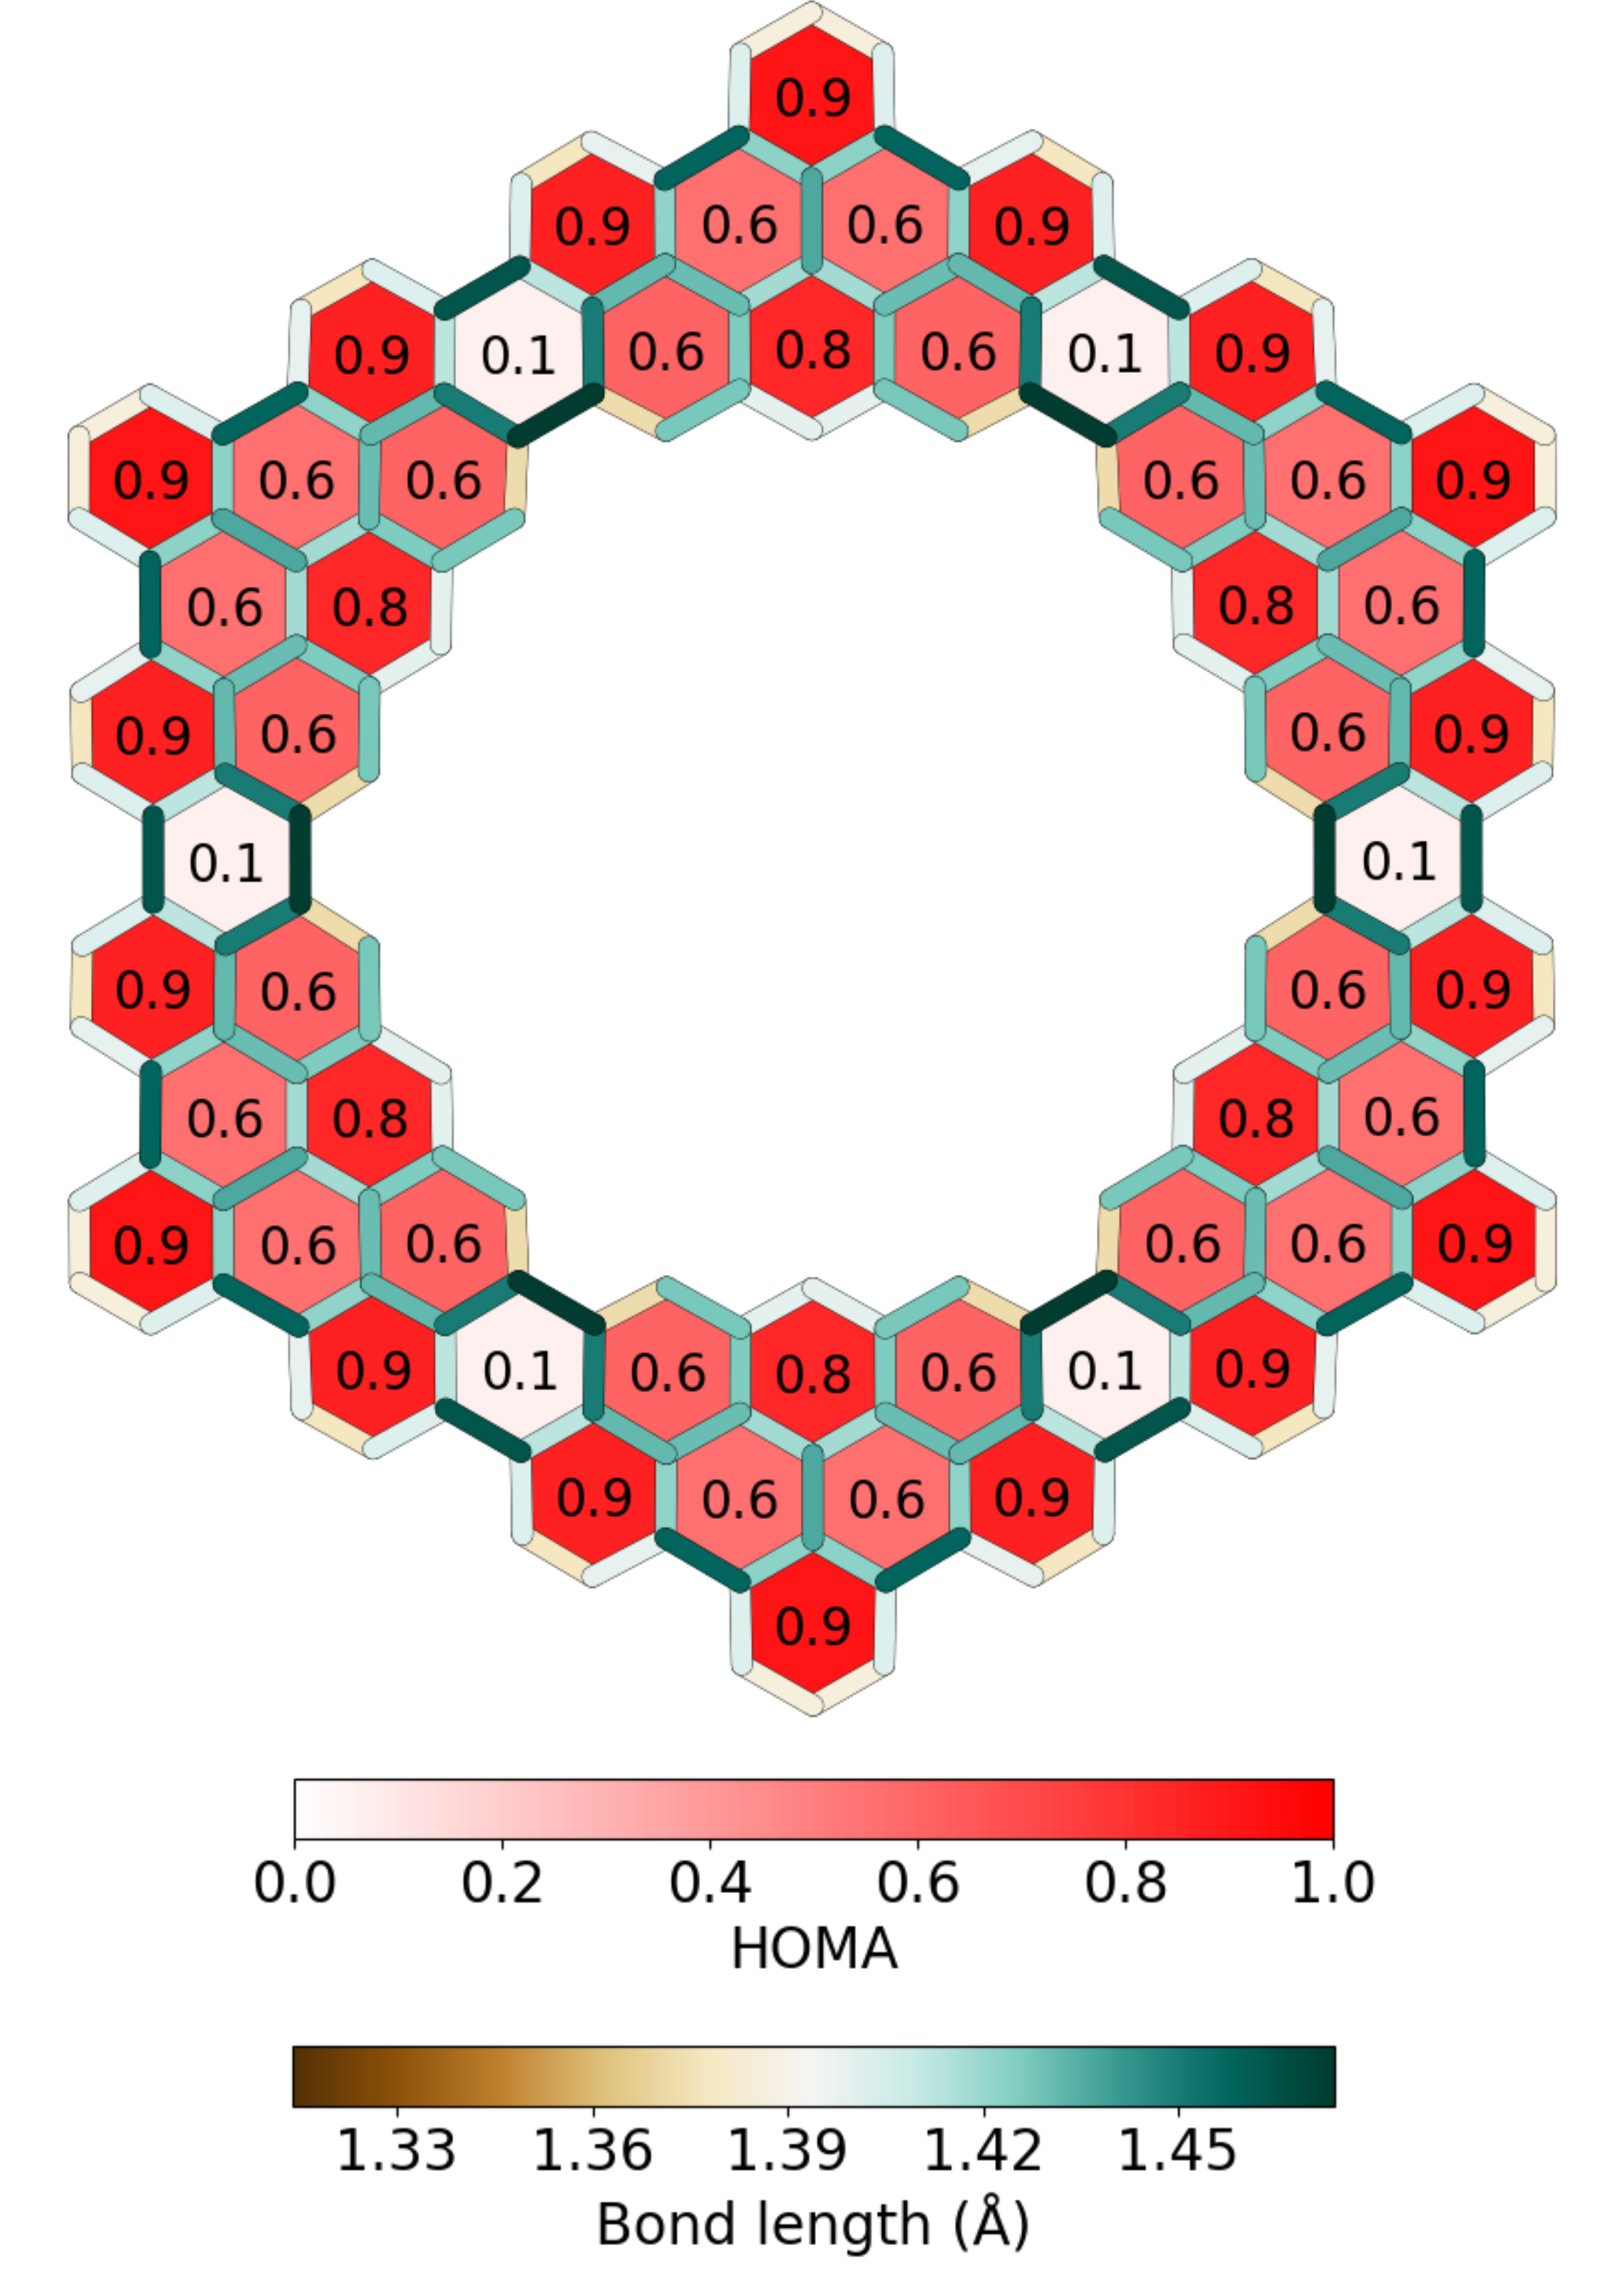
\includegraphics[width=0.65\textwidth]{images/geom.png}
	\end{center}
	\fonte{Autor(a).}
\end{figure}

\begin{figure}[htb]
\caption{\label{fig:HOMA2} Valores de HOMA para a estrutura do Kekuleno gerados com o \textit{Balmy.jl}.}
	\begin{center}
		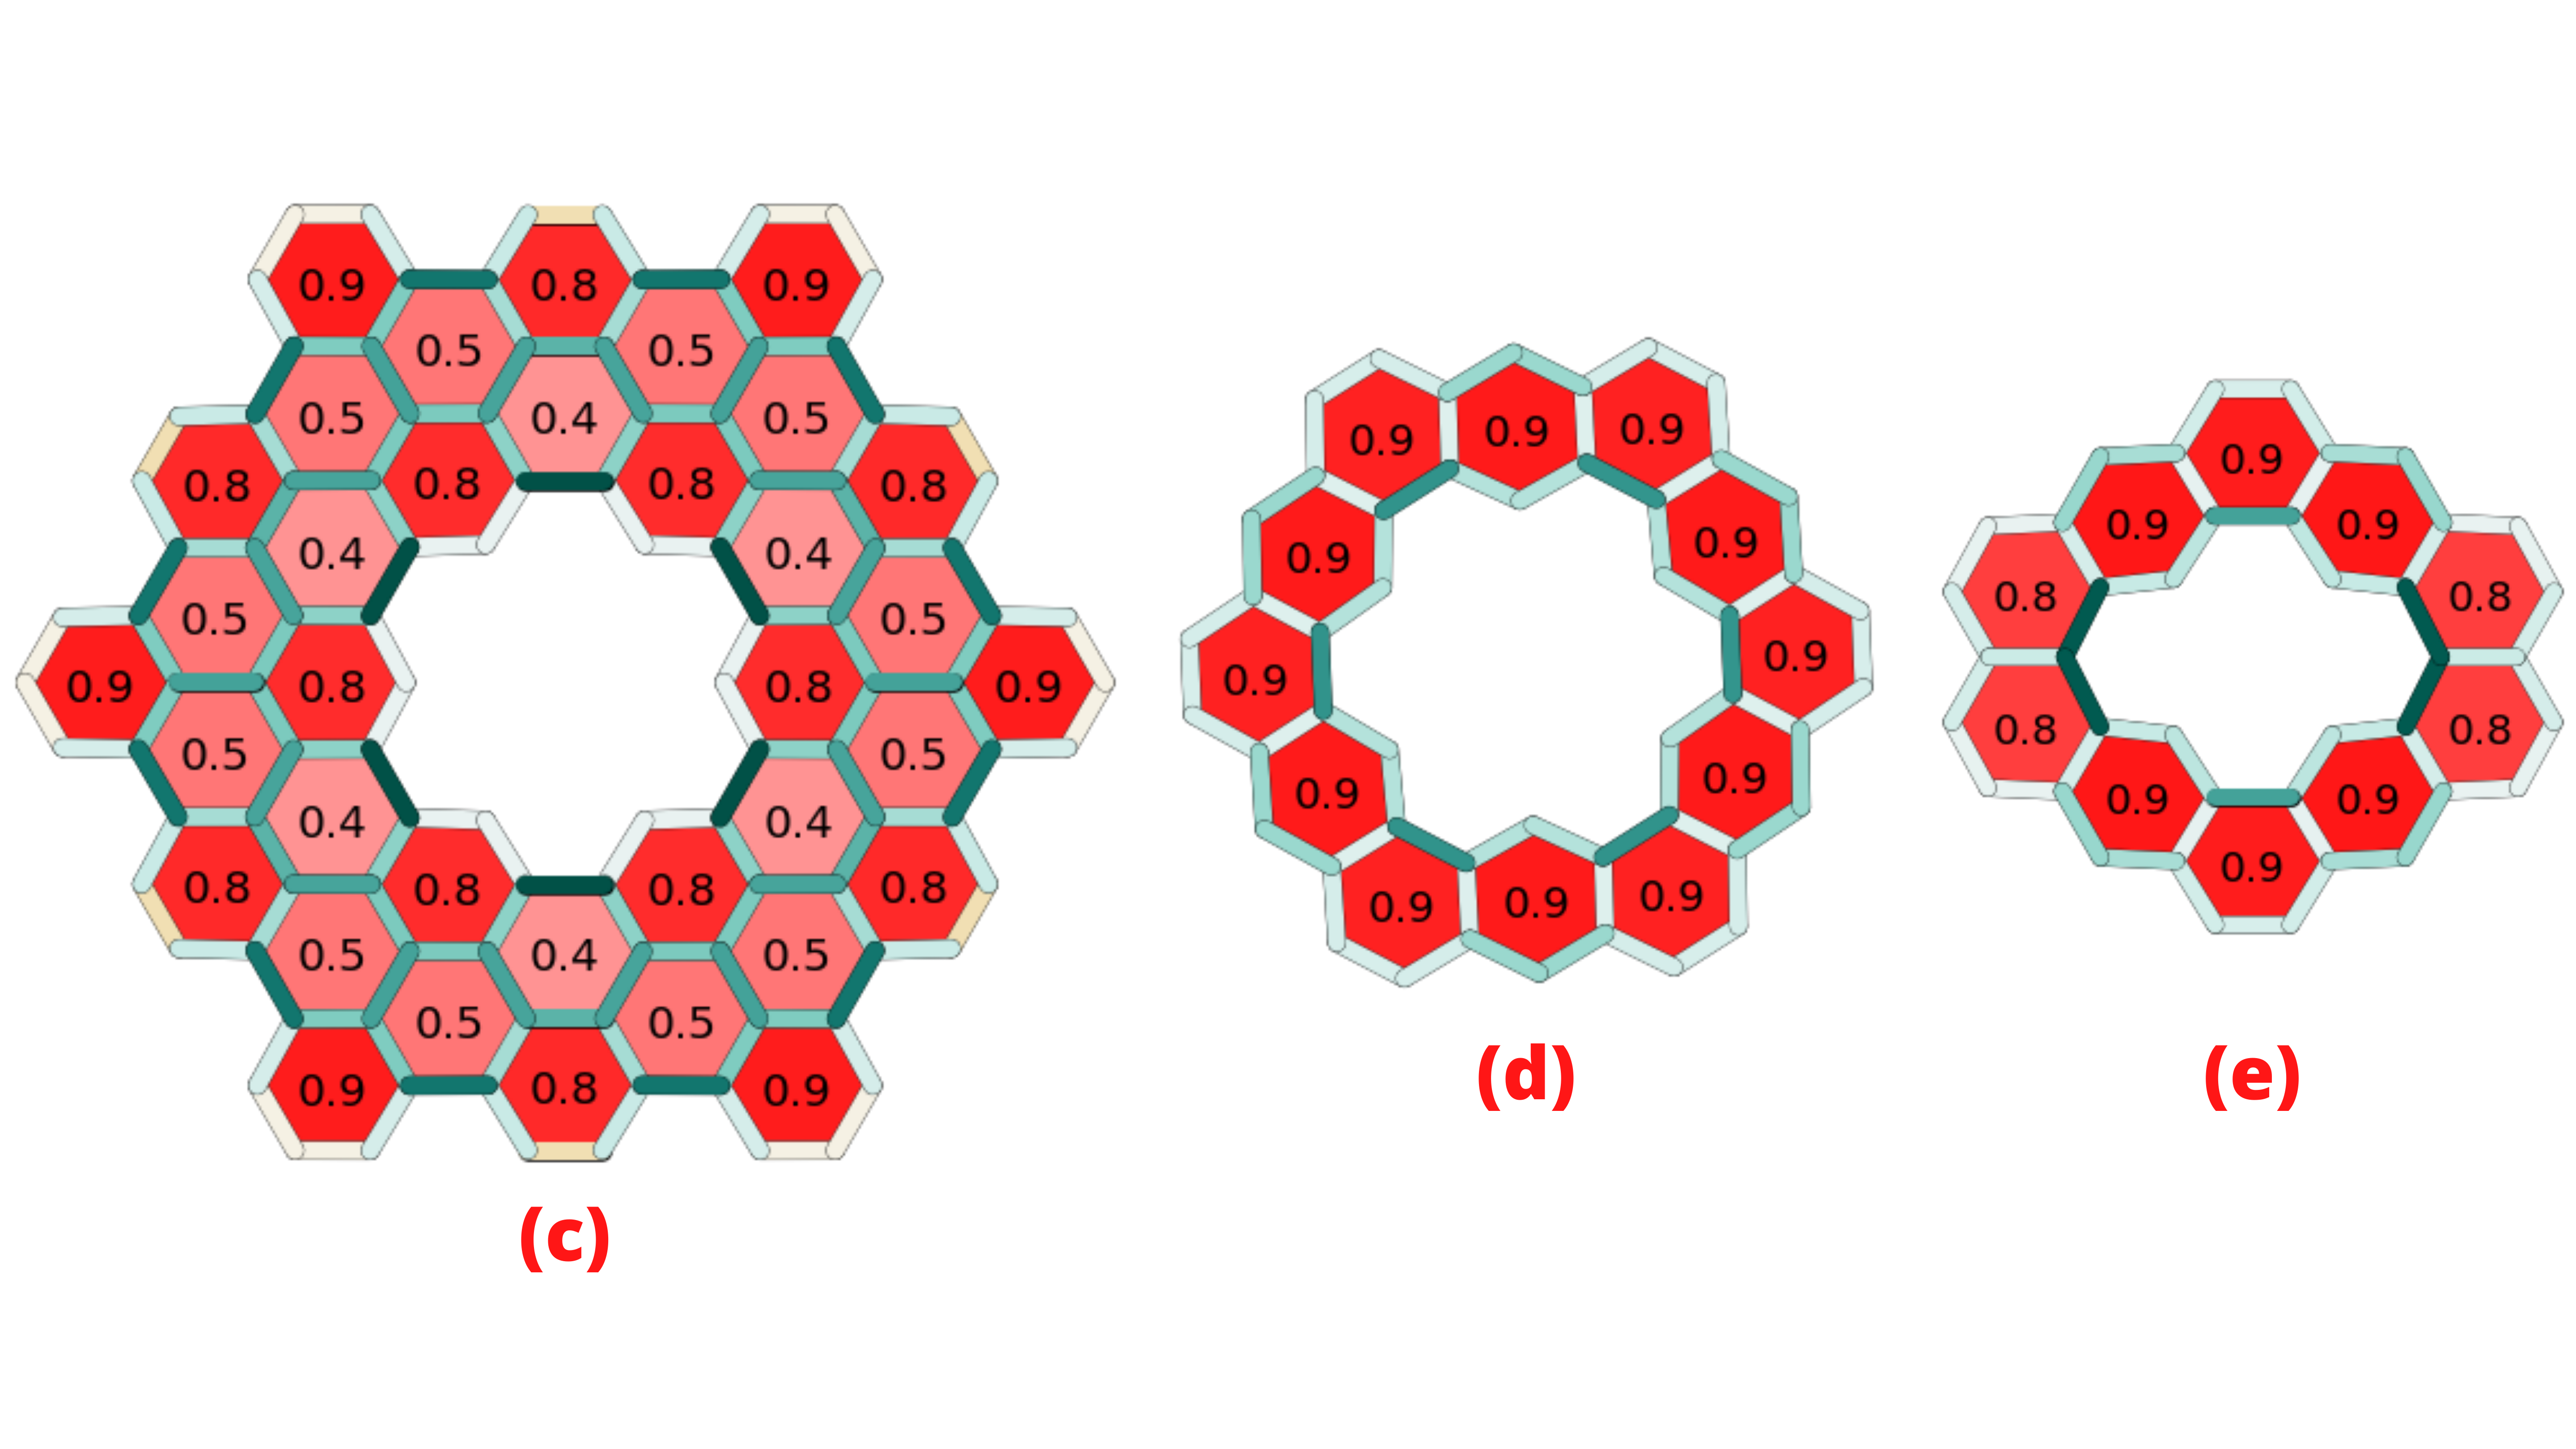
\includegraphics[width=1.0\textwidth]{images/15.png}
	\end{center}
	\fonte{Autor(a).}
\end{figure}

\subsection{Heterociclos aromáticos}

O efeito da ressonância em estruturas heterocíclicas depende da geometria do sistema e do tipo de heteroátomo presente no anel. No caso dos compostos que correspondem a anéis de cinco membros, como pirrol, furano, e seus derivados, são possíveis conjugações entre os pares de elétrons livres (do(s) heteroátomo(s)) e o sistema $\pi$. Consequentemente, são gerados híbridos de ressonância não equivalentes entre si, uma com separação de carga, e outra sem, não permitindo que a deslocalização eletrônica seja completa. Por outro lado, anéis de seis membros, a exemplo da piridina e seus derivados, apresentam conjugação $\pi-\pi$ total, com estruturas de ressonância que não têm separação de carga.

Após os efeitos de ressonância, os índices \gls{HOMED} (Tabela 11) calculados para as estruturas otimizadas do pirrol e do furano são inferiores aos dos heteroaromáticos de seis membros, como a piridina e o íon piranil, respectivamente. O índice \gls{HOMED} para o íon piranilíaco também é menor do que o índice para a piridina. Uma substituição do íon \ce{CH} pelo átomo N-aza em anéis com cinco membros parece reduzir o índice \gls{HOMED} em maior grau para O- que para N-derivados. Para anéis com seis membros, presença do átomo adicional N-aza em azinas não destrói o sistema de deslocalização completa de elétrons $\pi$ no sistema. Para os anéis de seis membros O-derivados, o índice \gls{HOMED} depende fortemente da posição do átomo N-aza. Ele diminui para posições 3 e 3,5; onde o átomo N pode estar próximo do átomo C+, e aumenta para a posição 4 onde o átomo N pode assumir a carga positiva.

\begin{figure}[htb]
\caption{\label{fig:HOMA3} Valores de HOMA para a estrutura do Kekuleno gerados com o \textit{Balmy.jl}.}
	\begin{center}
		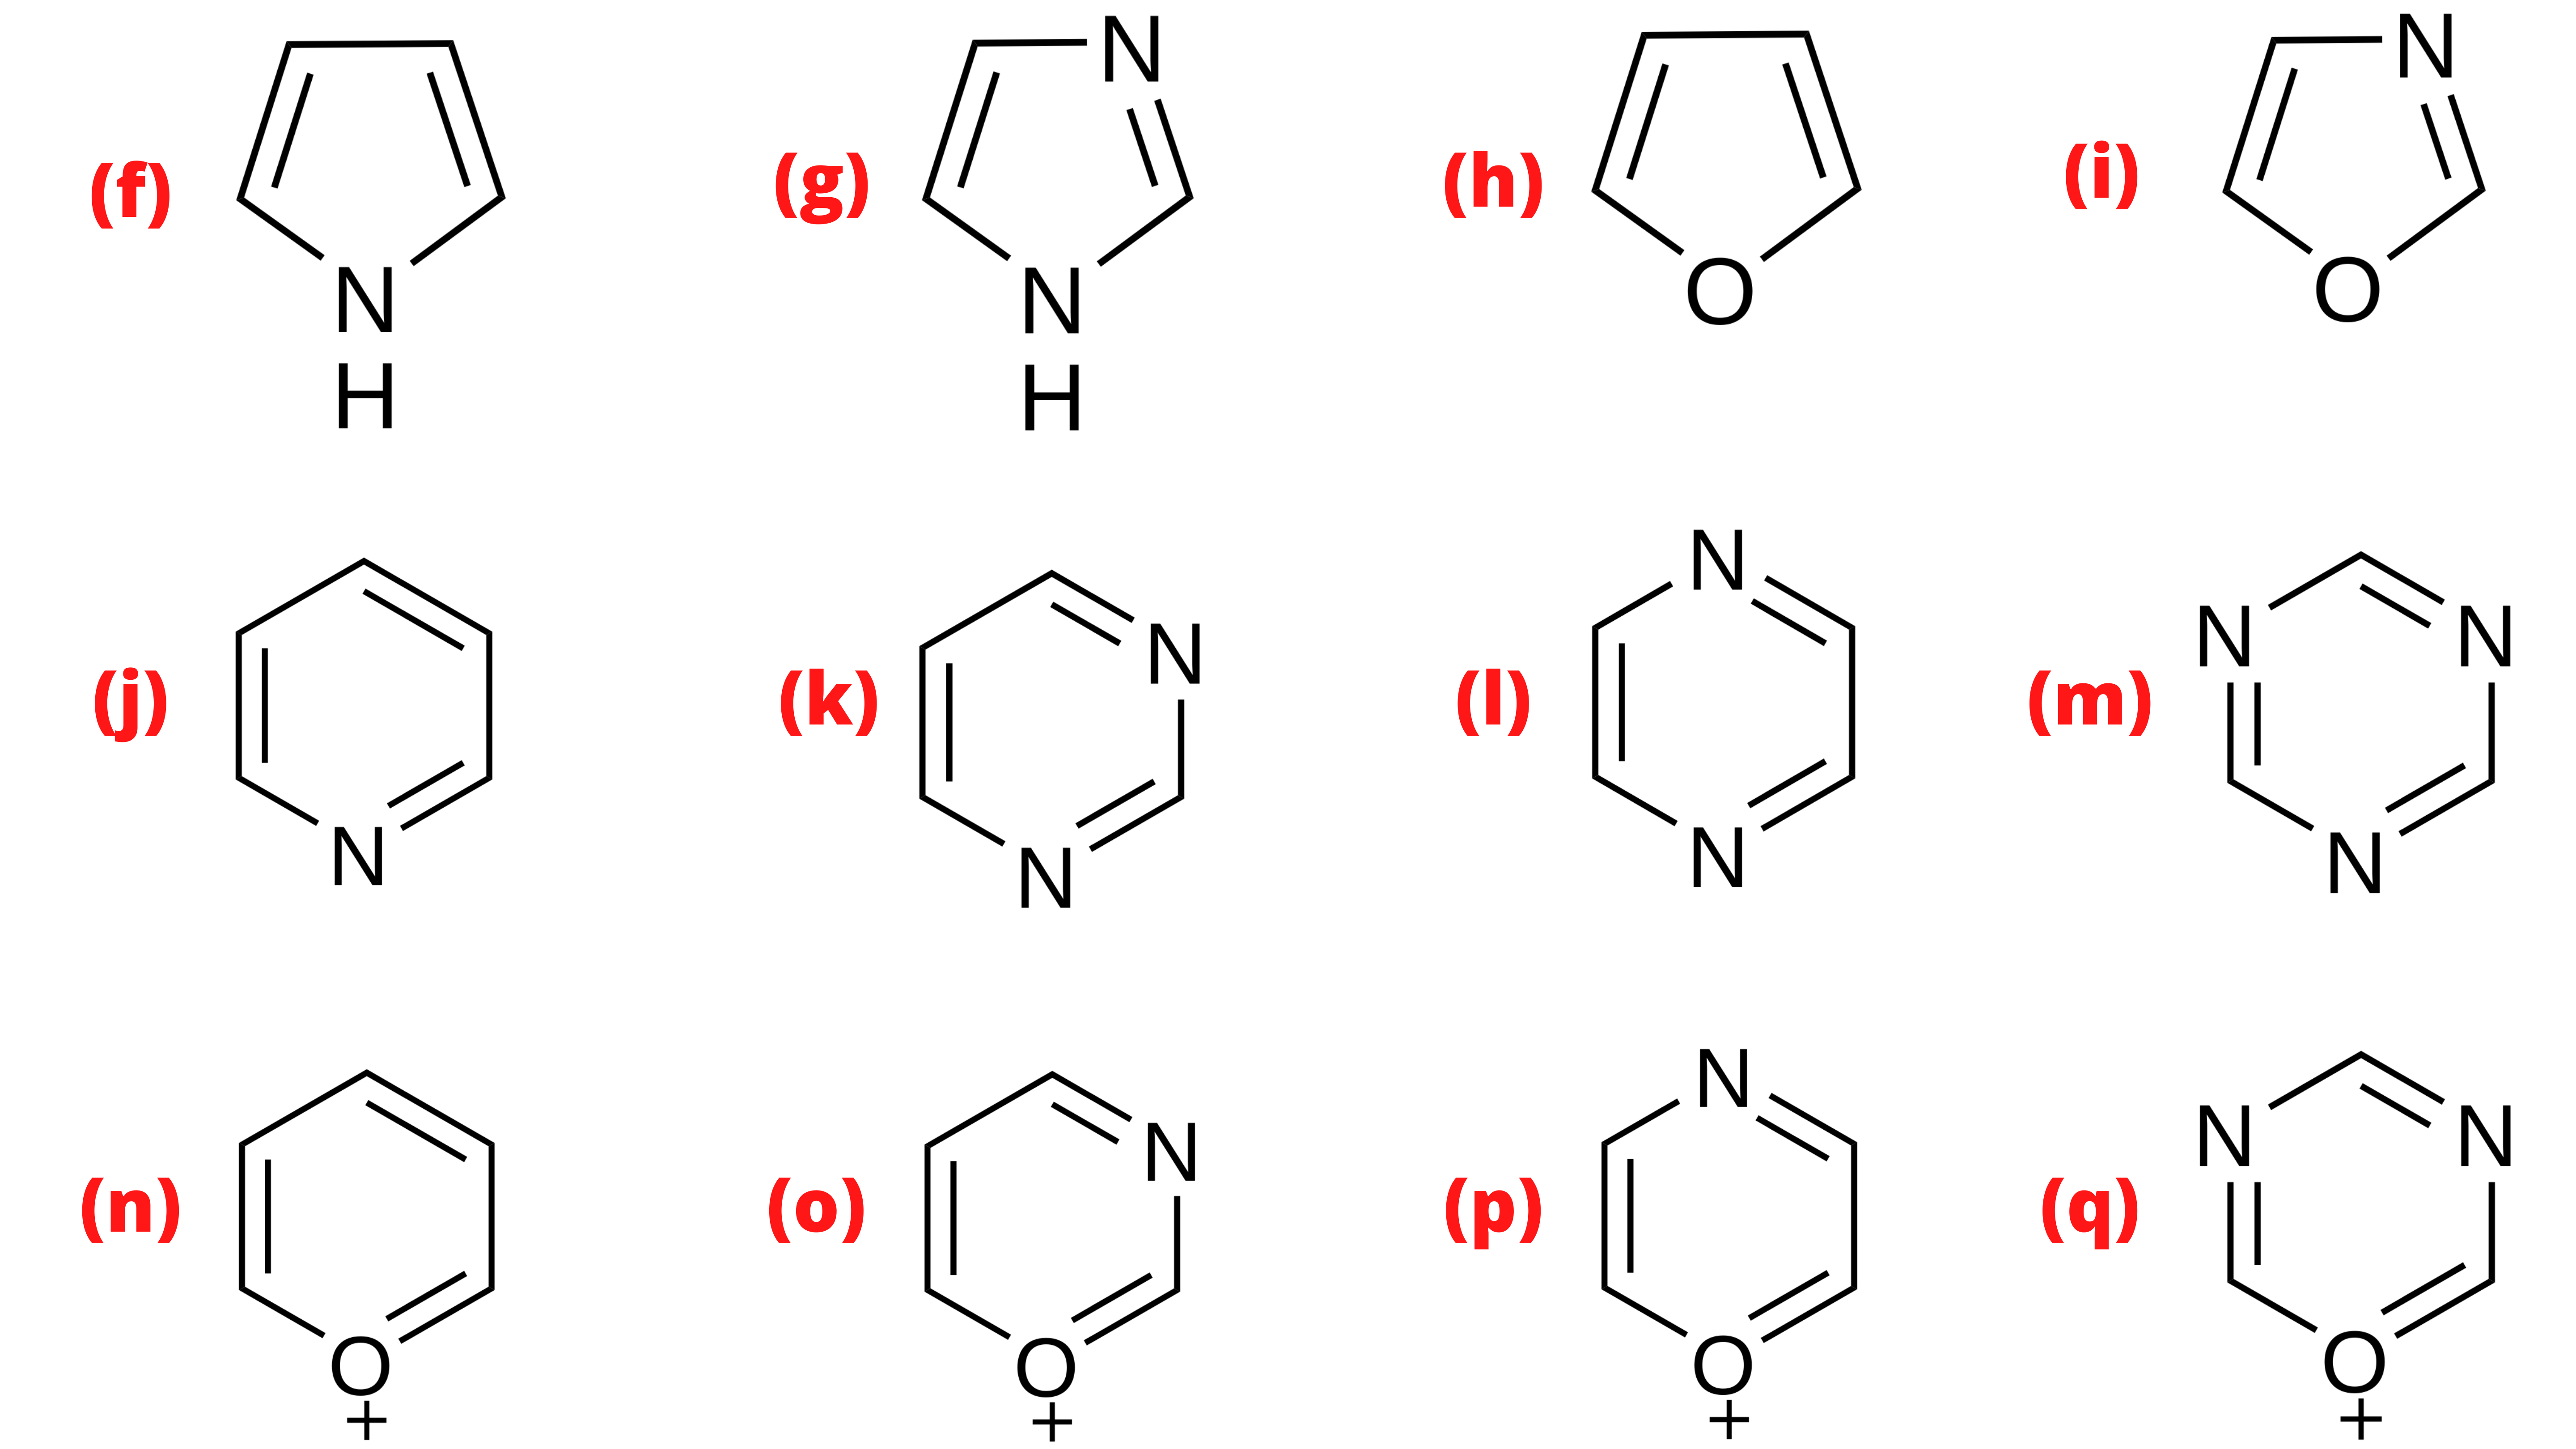
\includegraphics[width=1.0\textwidth]{images/fig2(7).png}
	\end{center}
	\fonte{Autor(a).}
\end{figure}

\begin{table}[htb]
	\centering
	\caption{\label{tab:homed/homa} Índices \gls{HOMED} e \gls{rHOMA} para sistemas simples heteroaromáticos.}
	\begin{tabular}{cccccc}
		\toprule
	\textbf{Molécula} & \gls{HOMED} & \textbf{Molécula} & \gls{HOMED} & \textbf{Molécula} & \gls{HOMED}
 \\
  & \gls{rHOMA} & & \gls{rHOMA} & & \gls{rHOMA}
 \\
		\midrule
    (\textbf{f}) & 0.921 & (\textbf{j}) & 0.9997 & (\textbf{n}) & 0.926 \\
    & 0.854 & & 0.995 & & 0.748 \\
    (\textbf{g}) & 0.903 & (\textbf{k}) & 0.9995  & (\textbf{o}) & 0.893 \\
    & 0.882 & & 0.999 & &  0.699 \\
    (\textbf{h}) & 0.749  & (\textbf{l}) & 0.9999 & (\textbf{p}) & 0.951 \\
    & 0.189 & & 0.996 & & 0.816 \\
    (\textbf{i}) & 0.702 & (\textbf{m}) & 1 (\textbf{padrão}) & (\textbf{q}) & 0.870  \\
    & 0.224 & & 1.000 & & 0.661 \\
    \bottomrule
	\end{tabular}
	\fonte{Autor(a).}
\end{table}

\section{Análise estatística}

Para além dos resultados já mostrados, ainda é possível discutir o porquê do índice \gls{HOMA} ser a melhor alternativa para trabalhar com a aromaticidade a nível geométrico. Matematicamente, podemos interpretar o \gls{HOMA} como uma função matemática de objetos como o quadrado da distância em um espaço molecular abstrato de dimensão $n$. Chamemos ele de \gls{MS}, no qual uma molécula pode ser representada por um ponto $X = (x_1, x_2, \cdots, x_n)$, onde as coordenadas subsequentes correspondem aos comprimentos da ligação \ce{CC} selecionada. Uma comparação entre duas moléculas, $X$ e $Y$, pode ser expressa como uma distância $d(X, Y) = \displaystyle \sqrt{\sum_{i=1}^{n} (x_i - y_i)^2}$ no \gls{MS}. 

Essa comparação também faz sentido se estivermos interessados somente em uma diferença entre os fragmentos restritos, como os anéis, para avaliar sua aromaticidade. É suficiente dizer que, nessa definição:

\begin{equation}
    HOMA = 1 - \textit{const} \cdot d^2(X, Y)
\end{equation}

\noindent onde $d(\cdot)$ corresponde à distância no \gls{MS}, $X$ é um anel em uma dada molécula e $Y = (y_1, y_2, \cdots, y_n)$ é o benzeno, no qual todas as coordenadas são iguais entre si: $y_1 = y_2 = \cdots = y_n = y = d(CC)$. É uma representação espacial do que seria o $R_{opt}$ na \autoref{eq:3}. Por outro lado, \textit{const} corresponde ao fator $\alpha / n$ da \autoref{eq:3}. Adicionalmente, se nós assumirmos que existe uma molécula $Y$ na qual $y_1 = y_2 = \cdots = y_m = y = d(CC_{benzeno})$, mas $m \neq 6$, então nós calculamos o \gls{HOMA} para qualquer molécula composta por um número arbitrário de átomos de carbono.

No campo da estatística, o $k$-ésimo momento central da função de probabilidade de uma variável aleatória $x$, $\mu_k$, ou seja, o $k$-ésimo grau do valor esperado, é definido como se segue: $\mu_k = \langle (x - \langle x \rangle)^k \rangle = \displaystyle \frac{1}{n} \sum_{i = 1}^n (x_i - \bar{x})^k$, onde $\langle \bullet \rangle$ e $\bar{x}$ denotam a média aritmética.
Desse modo, o $k$-ésimo momento, $m_k = \langle x^k \rangle = \displaystyle \frac{1}{n} \sum_{i=1}^n (x_i)^k$, não é tomado sobre a média e $\mu_2 = m_2 - m_1^2$.

Então, se $x_i$ é identificado como o i-ésimo comprimento $R_i$ em uma molécula (um anel) e $\bar{x}$ como o $R_{opt}$, então o índice \gls{HOMA} está conectado à variância, que é o segundo momento central para as múltiplas variáveis discretas aleatórias: $x_1, x_2, \cdots, x_n$, ou seja, 

\begin{equation}
\label{statistic}
\begin{split}
    HOMA = 1 - \alpha \bigg[\frac{1}{n} \sum_{i=1}^n (x_i - \bar{x})^2 \bigg] = 1 - \alpha \cdot \mu_2 \\ = 1 - \alpha \cdot (m_2 - m_1^2 )
\end{split}
\end{equation}

\noindent onde o $\alpha$ corresponde à mesma constante de normalização da \autoref{eq:3}. Notemos que a \autoref{statistic} permite que $n$ seja maior do que 6 porque pode ser compreendido como o número de comparações com o comprimento de ligação ótimo. Ou seja, o índice \gls{HOMA} pode ser calculado para qualquer molécula composto por um número arbitrário de ligações \ce{CC}.

Uma vez que o índice \gls{HOMA} pode ser expresso como uma função linear de $d^2$ ou $\mu_2$, uma descrição melhor da aromaticidade geométrica pode ser buscada entre as extensões do \gls{HOMA}, o que é tratado como uma distância abstrata ou um parâmetro estatístico. Aqui, será explorada a abordagem estatística.

\begin{equation}
    \Gamma = 100 \cdot (\mu_1^\circ + \mu_2^\circ + \mu_3^\circ + \mu_4^\circ)
\end{equation}

\noindent onde $\mu_k = \displaystyle \frac{\mu_k}{(m_{1, ref})^k}$ e $m_{1, ref}$ é a média na molécula de referência. Dividindo $\mu_k$ pelo $k$-ésimo. Dividir $\mu_k$ pela potência de $m_{1, ref}$ garante a adimensionlidade do índice $\Gamma$.